\chapter{Spin Zero}
\label{chap:spin-zero}

Our particle will be the simplest kind of particle: a \emphi{scalar boson} or \emphi{spin-zero particle}, whose only quantum number is momentum. The standard model --- the complete theory of particle physics --- contains one of these scalars in the form of the Higgs particle, though there are additional particles such as mesons which can be approximated as scalars, as we will later discuss.

The first step in creating this scalar is to write a Lagrangian for a field $\phi$ defined at every spacetime point $x$. Let's assume for now that the field takes on real values. Symmetries place the following severe limit the terms this Lagrangian may contain:
\begin{enumerate}
  \item Translations symmetry forbids terms that contain coordinates like $x$ or $t$
  \item Lorentz symmetry forces forbids uncontracted spacetime indices
  \item The Hamiltonian (and Lagrangian) must have a minimum energy so the field does not fly off to infinity
  \item If $\phi$ were complex, the fact that action is real would forbid any complex-valued term, which includes any odd power of $\phi$ 
\end{enumerate}

Furthermore, in the low energy regime where we might expect $\phi$ to be small (few particles present) and $\del_\mu \phi$ to be small (low momentum), we should not include terms which involve too many powers of $\phi$. The exact cutoff for how many powers is ``too many'' will be discussed later.

Given the above constraints on the Lagrangian, the only available terms to the Lagrange density $\mathcal{L}$ are
$$\phi\del_\mu \del^\mu \phi,\qquad
(\del_\mu \phi)(\del^\mu \phi),\qquad
\phi^2,\qquad\phi^3,\qquad
\phi^4,$$
and higher order terms. However, the first two terms are identical. This is because the QFT principle of least action (\ref{eqn:qft-least-action}) only involves $\int d^4 x\mathcal{L}$ rather than $\mathcal{L}$ directly. When under an integral, integration by parts guarantees that $\phi\del_\mu \del^\mu \phi=-(\del_\mu \phi)(\del^\mu \phi)$. For this reason, we drop the first term with no loss of generality. We also usually drop the last term, but we will add it back in for a later section.

% To make our particle simple, let us consider the following question. What happens to a state $\ket \psi$ when we swap two $\phi$ particles? Since all $\phi$ particles are equivalent, this swap cannot represent a physical change in $\ket \psi$, so the new $\ket \psi$ can differ only by an overall phase.

This discussion leaves us with only one possible action at low order:
\begin{e}
  \mathcal{L} = -\frac{1}{2}(\del_\mu \phi)^2 - \frac{m^2}{2}\phi^2 + \frac{\lambda}{4!} \phi^4.
  \label{eqn:scalar-lagrangian}
\end{e}
The constants $m^2$ and $\lambda$ were inserted to preserve generality, but no constant was inserted before the first term because such a constant can always be set to $1/2$ by rescaling $\phi$. Each term in (\ref{eqn:scalar-lagrangian}) as an intuitive meaning which we will briefly describe now, and the later sections will elucidate them in much greater detail.

\begin{enumerate}
  \item $-\frac{1}{2}(\del_\mu \phi)^2$ is known as the \emphi{kinetic term}, defined to be negative because, as will be seen later, if it were positive the $n$-point correlation functions would all diverge. This term encapsulates the kinetic energy of the particle because derivatives of fields represent momentum in much the same way that the quantum mechanical definition of the momentum operator $\hat{\bm p}$ is $i\bm \nabla$. The presence of two derivatives is akin to the $\bm p^2$ of kinetic energy.
  \item $\frac{m^2}{2}\phi^2$ is known as the \emphi{mass term}. Since $\phi^2$ is positive for any nonzero phi and is larger than any other power of $\phi$, this term controls the amount of energy that a particle contains merely by existing, and thereby increasing the local value of $\phi$. This inherent energy is defined as its mass. These first two terms of the Lagrangian are very similar to the Hamiltonian quantum harmonic oscillator, which has energies of $E = m(n+\frac{1}{2})$, where $n$ is an integer. Thus, energy can only increase in integer multiples of mass, which is an intuitive result. We will see that the same result occurs in quantum field theory.
  \item $\frac{\lambda}{4!}\phi^4$ is an \emphi{interaction term}. Since it is proportional to the square of the mass term, it represents two-body interactions, whereas $\phi^5$ would represent three-body interactions, etc. The presence of this term ruins the harmonic oscillator-like spectrum of $E = m(n+\frac{1}{2})$ because it generates potential energy when two particles are present in the same system. This is reminiscent one of the $1/r$ Coulomb potential of a charged particle, and indeed we will see that $\lambda \phi^4$ produces a $1/r$ potential between two $\phi$ particles.
\end{enumerate}

Encouragement to pursue (\ref{eqn:scalar-lagrangian}) comes from the fact that, if we set $\lambda=0$ and treat $\mathcal{L}$ as $\phi$ as a classical field theory, it produces the equation of motion
\begin{e}
  \del^\mu \del_\mu \phi^2 - m\phi^2 = 0
\end{e}
which is the famous Klein-Gordon equation mentioned in the introduction (\ref{eqn:klein-gordon}). It was already known to satisfy the laws of special relativity, and if $m=0$, it reduces to the familiar wave equation. The scalar Lagrangian (\ref{eqn:scalar-lagrangian}) is therefore a largely familiar beast.

\section{Solving the Scalar Path Integral Without Interactions}
\label{sec:scalar-free-path-integral}

In this section, we will solve for $n$-point correlation functions $\braket{\hat\phi(x_1)\cdots\hat\phi(x_n)}$ using the QFT principle of least action (\ref{eqn:qft-least-action}). We neglect the $\phi^4$ term by setting $\lambda=0$ in this section, but we will restore $\lambda$ in the following section. As such, the result of this section will be correlation functions for a non-interacting scalar theory.

Even with $\lambda=0$, evaluating the path integral is an intricate process that requires several new mathematical techniques. We introduce these techniques in this section, which ends with a formula for the $n$PCFs of non-interacting scalar theory. The physical meaning of this formula is discussed in the following section.

Plugging the scalar Lagrangian into (\ref{eqn:qft-least-action}),
\begin{e}
  \braket{0|\hat\phi(x_1)\cdots\hat\phi(x_n)|0} = \frac{\int \mathcal{D}\phi\, \phi(x_1)\cdots\phi(x_n)e^{-\frac{i}{2}\int d^4 x\brackets{-(\del_\mu\phi)^2 - m\phi^2}}}{{\int \mathcal{D}\phi\,e^{-\frac{i}{2}\int d^4 x\brackets{-(\del_\mu\phi)^2 - m\phi^2}}}}.
  \label{eqn:npcf-scalar}
\end{e}
The $\phi$ fields in the exponent are functions of $x$, but the $(x)$ has been suppressed for clarity.

It appears that if we can calculate the numerator for any $x_1 \dots x_n$, then we can calculate the denominator too and therefore any $n$PCF. We'll start with the case where $n=0$:
\begin{e}
  \int \mathcal{D}\phi\, e^{-\frac{i}{2}\int d^4 x\brackets{-(\del_\mu\phi)^2 - m\phi^2}}
\end{e}
Note that both terms in the exponent are quadratic in $\phi$. We can therefore separate the $\phi$s as follows:
\begin{e}
  \int \mathcal{D}\phi\, e^{-\frac{i}{2}\int d^4 x\, \phi^* \brackets{-\del^2 - m}\phi}.
  \label{eqn:gaussian-scalar}
\end{e}

(\ref{eqn:gaussian-scalar}) is a Gaussian integral because the exponent is quadratic in $\phi$. This makes it one of the only path integrals which can be solved analytically with perfect accuracy, and we will therefore spend considerable time on it. The next subsection is dedicated to evaluating it, while the following generalizes the result to $n \neq 0$. Following this, we will return to computing $n$PCFs.

\subsection{Infinite Dimensional Gaussian Integrals}
The Gaussianity of (\ref{eqn:gaussian-scalar}) can be seen more clearly if we consider a one-dimensional spacetime, broken up into a lattice with $N$ sites ans spacing $a$. In this case, $\phi(x_i)$ becomes $\phi_i$, $\int d^4x$ becomes $\sum_i a^4$ and $\del^2 \phi(x_i)$ becomes $(\phi_{i-1} + \phi_{i+1} - 2\phi_i) / a^2$. Furthermore, the path integral breaks down as an integral over each $\phi_i$, so that the entire function becomes
\begin{e}
  \prod_i^N\int d\phi_i\, e^{-\frac{i}{2}\sum_{jk}\, \phi_j^*M_{jk}\phi_k} = \prod_i^N\int d\phi_i\, e^{-\frac{i}{2}\bm \phi^\dagger M\bm \phi}
  \label{eqn:gaussian-scalar-matrix-form}
\end{e}
where
\begin{e}
  M_{ij} = -ma^4\delta_{ij} + a^2(\delta_{i,j+1} + \delta_{i,j-1} - 2\delta_{ij})
\end{e}
is a matrix. In the second equality (\ref{eqn:gaussian-scalar-matrix-form}), we have switched to matrix notation, where $\bm \phi$ is a vector of $\phi_i$. Inspection reveals that $M$ is Hermitian and therefore can be diagonalized as $M = U^\dagger \Lambda U$, where $U$ is a unitary matrix and $\Lambda$ is a diagonal matrix of eigenvalues $\lambda_i$. Thus, the path integral becomes
\begin{e}
  \int d^N\bm\phi\, e^{-\frac{i}{2}(U\bm \phi)^\dagger \Lambda (U\bm\phi)}
  = \int d^N\bm\phi\, e^{-\frac{i}{2}\phi^\dagger \Lambda \bm\phi} = \prod_i^N\brackets{\int d\phi_i\, e^{-\frac{i}{2}\phi_i^* \lambda_i \phi_i}}.
\end{e}
In the first equality we changed variables $\bm \phi \rightarrow U \bm \phi$, but since $\det U = 1$, doing so does not change the value of the integral. In the second equality we took advantage of the fact that $\Lambda$ is diagonal to integrate each component separately, leaving us with $N$ single-variable Gaussian integrals. It's a common fact that 
\begin{e}
  \int dx\, e^{-\alpha x^2}=\sqrt{\pi\alpha^{-1}}\qquad \mathrm{whenever}\qquad \Re \alpha > 0.
  \label{eqn:gaussian-1d}
\end{e}
Here, $\alpha = i\lambda_i/2$, and since $M$ is Hermitian, $\lambda$ is real and $\alpha$ is purely imaginary. We are therefore stuck on the edge of the validity of (\ref{eqn:gaussian-1d}). A common choice is to add a small imaginary number $i\epsilon$ to every eigenvalue so that $\Re \alpha$ is always slightly positive. Then our integral becomes
\begin{e}
  \prod_i^N\int d\phi_i\, e^{-\frac{i}{2}\sum_{jk}\, \phi_j^*M_{jk}\phi_k} = \frac{\pi^{N/2}}{\prod_i^N\sqrt{\lambda_i}} = \frac{\pi^{N/2}}{\sqrt{\det M}}.
\end{e}
The next step is to remove the discretization we performed at the beginning, by dividing spacetime into a lattice. This involves sending $N \rightarrow \infty$ and also changing $\det M$ such that the value of the above integral may become infinite. This is worrying, but not catastrophic, since the $n$PCFs of (\ref{eqn:npcf-scalar}) are all \textit{ratios} of gaussian integrals. If the $\pi^{N/2}/\sqrt{\det M}$ is common to both the numerator and the denominator, it will cancel out regardless of whether it is infinite.

The next step is therefore to generalize our Gaussian integral result to $n\neq 0$ so that we can confirm this cancellation in the $n$PCFs.


\subsection{Wick's Theorem}
\label{sec:wicks-theorem}

The last barrier preventing us from evaluating the properties of non-interacting scalar theory is the integral
\begin{e}
  \int \mathcal{D}\phi\, \phi(x_1)\dots\phi(x_n)e^{-\frac{i}{2}\int d^4 x\, \phi^* \brackets{-\del^2 - m}\phi}.
  \label{eqn:n-point-gaussian-integral}
\end{e}
We'll use a trick to solve this problem. First, we'll discretize spacetime as we did in the previous section:
\begin{e}
  \prod_i^N \int d\phi_i\, \phi_{j_1}\dots\phi_{j_n} e^{-i\, \bm\phi^\dagger M\bm \phi}.
\end{e}
where $\phi_{j_1}$ is the discretized $\phi(x_1)$. This integral can be solved more easily via the \emphi{generating function}
\begin{e}
  Z(\bm J) = \prod_i^N \int d\phi_i\, e^{-i\, \bm\phi^\dagger M\bm \phi + \bm J \cdot \bm \phi}
  \label{eqn:generating-function}
\end{e}
where $\bm J$ is an arbitrary vector. This function exists only to be differentiated, since
\begin{e}
  \eval{\frac{d^2Z}{dJ_{j_1}dJ_{j_2}}}_{\bm J = 0} = \prod_i^N \int d\phi_i\, \phi_{j_1}\phi_{j_2}e^{-i\, \bm\phi^\dagger M\bm \phi}
  \label{eqn:2pcf-to-gen-func}
\end{e}
which can be seen by explicitly differentiating (\ref{eqn:generating-function}). This derivative is clearly useful, since it is the integral need for a 2PCF. We therefore go about finding $Z(\bm J)$ via the same method as in the previous section:
\begin{es}
  Z(\bm J) &= \int d \bm \phi\, e^{-i\brackets{(U\bm\phi)^\dagger \Lambda(U\bm \phi) + \bm (U\bm J)^\dagger (U\bm \phi)}}\\
  &= \prod_i \brackets{\int d \phi_i\, e^{-i\brackets{\phi^*_i \lambda_i \phi_i + (U\bm J)_i^* \phi_i}}}\\
  &= \prod_i \brackets{\int d \phi_i\, e^{-i\, \abs{\phi_i\sqrt{\lambda_i} + \frac{(U\bm J)_i^*}{2\sqrt{\lambda_i}}}^2}e^{i\frac{|U\bm J|_i^2}{4\lambda_i}}}\\
  &= \prod_i \brackets{\sqrt{\frac{\pi}{\lambda_i}} e^{i\frac{|U\bm J|_i^2}{4\lambda_i}}}\\
  &= \frac{\pi^{N/2}}{\det M}e^{\frac{i}{4}\sum_i\Lambda^{-1}_i|U\bm J|_i^2} = \frac{\pi^{N/2}}{\det M}e^{\frac{i}{4}\bm J^\dagger U^\dagger \Lambda^{-1}U \bm J}\\
  &= \frac{\pi^{N/2}}{\det M}e^{\frac{i}{4}\bm J^\dagger M^{-1} \bm J}
  \label{eqn:partition-calculation}
\end{es}
where the first equality is true by diagonalizing the Hermitian matrix $M$, the second by substitution of variables, the third by completing the square, the fourth by substitution of variables again and evaluating the Gaussian integral, and the rest by rearranging the equation. This calculation revealed two crucial properties: (1) that $Z(\bm J)$ has the same infinite prefactor that the original Gaussian integral in the last section had, and (2) this prefactor is multiplied by a simple term containing $M^{-1}$. This term is simple enough that its derivative can be easily computed:
\begin{e}
  \eval{\frac{d^2Z}{dJ_{j_1}dJ_{j_2}}}_{\bm J = 0} = Z(0)M_{j_1j_2}^{-1}.
  \label{eqn:2pcf-wick}
\end{e}

Higher derivatives are also simple: two more derivatives multiplies the above by$M_{j_3j_4}^{-1}$. However, since derivatives commute, $Z(0)M_{j_1j_2}^{-1}M_{j_3j_4}^{-1}$ cannot be the only term. The value of the integral must be symmetric under all permutations of the indices. Therefore,
\begin{e}
  \eval{\frac{d^2Z}{dJ_{j_1}dJ_{j_2}dJ_{j_3}dJ_{j_4}}}_{\bm J = 0} = Z(0)\parens{M_{j_1j_2}^{-1}M_{j_3j_4}^{-1} + M_{j_1j_3}^{-1}M_{j_2j_4}^{-1} + M_{j_1j_4}^{-1}M_{j_2j_3}^{-1}}.
\end{e}

For $n$-many derivatives with $n$ even, there are $(n)!$ terms where each term represents one possible way to pair all the indices up. This rule for evaluating Gaussian integrals is called \emphi{Wick's theorem}.\footnote{Problem 1 is to prove this fact by induction.} If $n$ is odd, there are no ways to pair up the indices and the value of the Gaussian integral is zero. This can also be seen by noticing that the Gaussian is an even function, and an odd number of derivatives applied to an even function is an odd function which will take the value zero at $\bm J = 0$.

Remembering the connection between $Z$ and the PCFs, as in (\ref{eqn:2pcf-to-gen-func}), Wick's theorem states that 

\begin{e}
  \braket{0|\hat\phi(x_{j_1})\cdots\hat\phi(x_{j_{2n}})|0} = \sum_{\mathrm{pairs}\ (a,b)_i\ \mathrm{of\ indices}}M_{a_1b_1}^{-1}M_{a_2b_2}^{-1}\dots M_{a_nb_n}^{-1}.
  \label{eqn:wick-discrete}
\end{e}

We have successfully computed our first $n$PCF! The next section is devoted to returning to a continuous, four-dimensional spacetime, after which we will discuss the consequences of this $n$PCF.

\subsection{Continuous Spacetime Gaussian Integrals}
When spacetime is continuous, the matrix $M$ used profusely in the preceding sections does not make sense, meaning that the $M^{-1}$ of Wick's theorem is not defined. For scalar the free theory, we had $\mathcal{L} = \phi^*(-\del^2 - m^2) \phi / 2$, so the analog of the matrix $M$ will be the differential operator $O_x = (-\del^2 - m^2)/2$, where the subscript $x$ indicates that $O$ contains derivatives with respect to $x$. The analog of $M^{-1}$ is the function $G(x,y)$ which satisfies
\begin{e}
  O_x G(x, y) = \delta(x-y).
\end{e}
This is analogous to the definition of a matrix inverse, which is that 
\begin{e}
  M_{ij} M^{-1}_{jk} = \delta_{ik}.
\end{e}
The function $G(x, y)$ is called the Green's function for operator $O$ and must be computed for each $O$ that may appear. Computing a Green's function for an arbitrary operator is generally difficult, but our operator $O_x = (-\del^2 - m^2)$ has translation symmetry, which makes its Green's function easier to compute. Translation symmetry is manifested in the fact that $O_x$ not a function of $x$, but we could have also guessed it would appear from the fact that the Lagrangian density from which $O_x$ is derived had to be translation invariant. This symmetry requires that $G$ must also be translation invariant, so that $G(x,y) = G(x-y_0,y-y_0)$ for any $y_0$. Choosing $y_0=y$ allows us to write $G(0, x-y)$, or $G(x-y)$ if we drop the first argument. Thus, the new definition of the Green's function can be simplified to
\begin{e}
  O_z G(z) = \delta(z)
  \label{eqn:greens-function-translated}
\end{e}
for $z=x-y$.

Translational symmetry allows us to solve for $G_x$ via the Fourier transform. Let's define the Fourier transform of $G(z)$ as
\begin{e}
  G(k) = \int d^4 z\, e^{-ik\cdot z} G(z), \qquad G(z) = \int \ftve{4}{k} e^{ik\cdot z} G(k), .
\end{e}
We must also transform $O_x$ such that it can operate on $G(k)$. Constants such as $m$ are unaffected by a Fourier transform, but derivatives such as $\del_\mu$ do transform:
\begin{e}
  \del_\mu f(x) = \int \ftve{4}{k} \del_\mu e^{ik\cdot x}f(k) = \int \ftve{4}{k} ik_\mu e^{ik\cdot x}f(k).
\end{e}
These two substitutions for $G(x)$ and $\del_\mu$ transform (\ref{eqn:greens-function-translated}) to
\begin{e}
  \int \ftve{4}{k}\parens{k^2 - m^2}G(k) = \delta(z).
  \label{eqn:scalar-greens-partway}
\end{e}
A property of the $\delta$ function is 
\begin{e}
  \delta(z) = \int \ftve{4}{k} e^{ik\cdot z}.
\end{e}
Substituting this property into (\ref{eqn:scalar-greens-partway}) causes the $k$ integral to appear on both sides of the equation. Removing it, we get
\begin{e}
  (k^2 - m^2) G(k) = 1 \implies G(k) = \frac{1}{k^2 - m^2}.
  \label{eqn:scalar-propagator-momentum}
\end{e}

This concludes our calculation of the Green's function. The analog of Wick's theorem (\ref{eqn:wick-discrete}) for Green's functions is 
\begin{e}
  \braket{0|\hat\phi(x_{1})\cdots\hat\phi(x_{2n})|0} = \sum_{\mathrm{pairs}\ (a,b)_i\ \mathrm{of\ indices}}G(x_{a_1}-x_{b_1})\dots G(x_{a_n}-x_{b_n}).
  \label{eqn:wicks-theorem}
\end{e}
and $n$PCFs with $n$ odd are zero.

\subsection{Putting the Pieces Together}

In order to use our momentum-space Green's function (\ref{eqn:scalar-propagator-momentum}) we must Fourier transform the $n$PCF:
\begin{es}
  \braket{0|\hat\phi(k_{1})\cdots\hat\phi(k_{2n})|0} =& \int d^4x_1\dots d^4x_{2n}\,\parens{e^{ik_1\cdot x_1}\dots e^{ik_{2n}\cdot x_{2n}}}\\
  &\times\braket{0|\hat\phi(x_{1})\cdots\hat\phi(x_{2n})|0}\\
  =&\int d^4x_1\dots d^4x_{2n}\,\parens{e^{ik_1\cdot x_1}\dots e^{ik_{2n}\cdot x_{2n}}}\\
  &\times\sum_{\mathrm{pairs}\ (a,b)_i}G(x_{a_1}-x_{b_1})\dots G(x_{a_n}-x_{b_n})\\
  =&\sum_{\mathrm{pairs}\ (a,b)_i}\int d^4x_1\dots d^4x_{2n}\,\parens{e^{ik_1\cdot x_1}\dots e^{ik_{2n}\cdot x_{2n}}}\\
  &\times G(x_{a_1}-x_{b_1})\dots G(x_{a_n}-x_{b_n})
\end{es}
where the second equality came from applying Wick's theorem and the third commuted the sum over pairs to the front of the equation. We can now perform a unitary change of variables. For each Wick pairs of indices $(a,b)_i$, we define $y_i=(x_{a_i}+x_{b_i})/2$ and $z_i=x_{a_i}-x_{b_i}$, so that $d^4 x_{a_i}d^4x_{b_i} = d^4 y_id^4z_i$. The advantage of this transformation is that $G(x_{a_i}-x_{b_i})$ is now merely $G(z_i)$ and does not depend on $y_i$. The exponents also transform:
\begin{e}
  e^{ik_{a_i}\cdot x_{a_i}}e^{ik_{b_i}\cdot x_{b_i}} = e^{ip_i\cdot y_i} e^{i\ell_i \cdot z_i}
\end{e}
where $p_i = k_{a_i} + k_{b_i}$ and $\ell_i = (k_{a_i} - k_{b_i})/2$. The result is
\begin{es}
  \braket{0|\hat\phi(k_{1})\cdots\hat\phi(k_{2n})|0} &=\sum_{\mathrm{pairs}\ (a,b)_i}\prod_{i=1}^{n}\int d^4y_i d^4z_i\,e^{ip_i\cdot y_i} e^{i\ell_i \cdot z_i}G(z_i)\\
  &=\sum_{\mathrm{pairs}\ (a,b)_i}\prod_{i=1}^{n}(2\pi)^4\delta(p_i)G(\ell_i).
  \label{eqn:separable-gaussian-lagrangian}
\end{es}
The $\delta(p_i)$ term is nonzero only when $k_{a_i} = -k_{b_i}$, in which case $\ell_i = (k_{a_i}-k_{a_i})/2 = k_{a_i}$. Thus,
\begin{e}
  \braket{0|\hat\phi(k_{1})\cdots\hat\phi(k_{2n})|0} =\sum_{\mathrm{pairs}\ (a,b)_i}\prod_{i=1}^{n}(2\pi)^4\delta(k_{a_i} + k_{b_i})G(k_{a_i}).
  \label{eqn:momentum-npcf}
\end{e}
This result is actually valid for any quadratic Lagrangian, even ones which are not the free scalar lagrangian. Plugging in the Green's function for a scalar field,
\begin{e}
  \braket{0|\hat\phi(k_{1})\cdots\hat\phi(k_{2n})|0} =\sum_{\mathrm{pairs}\ (a,b)_i}\prod_{i=1}^{n}(2\pi)^4\frac{\delta(k_{a_i} + k_{b_i})}{k_{a_i}^2 - m^2}.
  \label{eqn:scalar-theory-npcf}
\end{e}
This is our first ever $n$PCF, computed exactly assuming the QFT principle of least action (\ref{eqn:qft-least-action}) and the scalar Lagrange density (\ref{eqn:scalar-lagrangian}). It depends only on the mass of the $\phi$ particle $m$ (included in the form of $G(k)$) and the $k$ values chosen to evaluate the $n$PCF at. In the next section, we will interpret the physical implications of this $n$PCF formula and show that it has both quantum mechanical and relativistic properties, confirming our hope that the QFT principle of least action would lead to a relativistic quantum theory. We will also discuss the spectrum of the 2PCF using the framework discussed in chapter \ref{chap:spectrum}, showing that the 2PCF indeed contains arbitrarily many particles of mass $m$.


\section{The Spin Zero Free Theory Is Quantum Mechanical and Relativistic}
The $n$PCFs of (\ref{eqn:scalar-theory-npcf}) have several crucial properties which are necessary for a relativistic quantum theory, which we enumerate below.

\paragraph*{Mass Energy Equivalence}
(\ref{eqn:scalar-theory-npcf}) enforces the relativistic $k^2 = m^2$ constraint due to the $k^2 - m^2$ in the denominator of the Green's function. This causes the $n$PCFs to be much greatest near $k^2 = m^2$ --- that is, the probability for a particle with momentum $k$ to be produced is greatest for $k^2 = m^2$ and much smaller elsewhere.

\paragraph*{Quantized Amplitude}
The $n$PCFs also show that a field $\hat \phi(k)$ at a given momentum $k$ cannot be arbitrarily rescaled. Since $m$ is constant and $k^2 = m^2$ as discussed above, there is no freedom to choose an arbitrary amplitude for $\phi$ and obey the (\ref{eqn:scalar-theory-npcf}). That is, the amplitude of $\phi$ is quantized. This is unlike a classical field theory such as electromagnetism, where the $\bm E$ field may take on whatever amplitude it wishes. But in any quantum mechanical theory, we expect the properties of particles to be quantized, with values such as field amplitude taking on only discrete values.

\paragraph*{No Scattering in Free Theory}
Chapter \ref{chap:scattering} outline a toolkit to use $n$PCFs to compute scattering cross-sections. It interpreted $\braket{0|\hat\phi(p_1)\hat\phi(p_n)\cdots\hat\phi(-q_1)\hat\phi(-q_m)|0}$ as the amplitude of scattering $n$ particles from momentum $p_i$ to $m$ particles of momentum $q_i$. (\ref{eqn:scalar-theory-npcf}) shows that this amplitude is zero except when the momentum can be paired up as $p_i = q_i$. Each pair adds the same factor to the correlation function due to the quantization of amplitude. This $p_i = q_i$ requirement shows that the free theory $n$PCFs do not allow particles to change momentum, even when other particles are present. This is equivalent to requiring no interactions, which is the definition of a free theory.

\paragraph*{Mass Spectrum of a Particle}
In chapter \ref{chap:spectrum}, we discussed the 2PCF in particular and showed that it is expected to have a pole at $k^2 = m^2$ where $m$ is the mass of any particle in the theory. We also showed that branch cuts where the 2PCF is infinite represent interaction cross-sections. Our 2PCF contains a pole at $k^2 = m^2$, where $m$ is the mass of the $\phi$ particle, exactly as expected. This is the only pole and there are no branch cuts, indicating again that this theory contains no interactions.

\paragraph*{Causality}
A founding principle of relativity is that information cannot be translated faster than the speed of light. If (\ref{eqn:scalar-theory-npcf}) is to be taken seriously as a theory of physics, we should expect $\hat\phi(x)$ to be uncorrelated with $\hat\phi(y)$ as long as $x$ and $y$ are spacelike-separated. Thus,
\begin{e}
  \braket{0|\hat\phi(x)\hat\phi(y)|0} = 0\qquad \mathrm{whenever} \qquad |\bm x - \bm y| > |x_0 - y_0|.
\end{e}
To check this, we will Fourier transform the 2PCF
$$
\braket{0|\hat\phi(k)\hat\phi(-k)|0} =(2\pi)^4\frac{\delta(0)}{k^2 - m^2}
$$
back into position space and check this fact. If we translate to $y=0$ and rotate until $x^\mu = (t,x,0,0)$, then
\begin{es}
  \braket{0|\hat\phi(x)\hat\phi(0)|0} &=\int \ftve{4}{k}e^{ik\cdot x}\frac{(2\pi)^4}{k^2 - m^2} \\
  &=\int d^3 \bm k\int dk^0 \, \frac{e^{-ik_0t + ik_1x}}{k_0^2 - \bm k^2- m^2}.
  \label{eqn:2pcf-integral-halfway}
\end{es}
The integrand contains a pole at $k_0^2 = \bm k^2 + m^2$, making the Fourier transform undefined. However, if we add a small $i\epsilon$ term into the denominator where $\epsilon>0$ is small, we can move the pole off the real axis and out of the way of the integration without changing the value of $G(k)$ very much. Defining $E^2 = \bm k^2 + m^2 > 0$, we must now solve\footnote{$E^2 = \bm k^2 + m^2$ is actually the energy of a particle with mass $m$ and momentum $\bm k$, but we will not need this fact.

Furthermore, in this equation we redefine $\epsilon$ on the right hand side to absorb its coefficients, which is allowed since $\epsilon$ is assumed to be small enough that it remains small even when multiplied by a finite number.}
\begin{e}
  I = \int dk^0 \, \frac{e^{-ik_0t}}{k_0^2 - E^2 - i \epsilon} = \int dk^0 \, \frac{e^{-ik_0t}}{2E}\parens{\frac{1}{k_0 - E + i \epsilon} - \frac{1}{k_0 + E - i\epsilon}}.
\end{e}
This integral is performed over $z\in(-\infty, \infty)$, but we can always add more to the contour of integration (even extending it into the complex plane) as long as the value of the integrand on that contour is zero. For $t>0$, $e^{-ik_0 t}$ is small whenever $\Im k^0 \ll 0$ and for $t>0$ the condition is $\Im z \gg 0$. We therefore choose to extend the contour in a large arc around the complex plane, below the real axis for $t>0$ and above it for $t<0$ (Figure \ref{fig:epsilon-complex-plane}). Since this new contour is closed, we may use the Residue Theorem (see chapter \ref{chap:complex-analysis}) to evaluate it, picking up the $-E$ pole when closing the curve above the real line, and the $+E$ pole when closing the curve below the real line. Thus,
\begin{e}
  I = \begin{cases}
    \pi i\frac{e^{-itE}}{E}& \mathrm{for} \ t>0\\
    -\pi i\frac{e^{itE}}{E}& \mathrm{for} \ t<0\\
  \end{cases}
\end{e}
The only difference between the $t>0$ and $t<0$ cases is an overall sign, which we ignore.

\begin{figure}
  \centering
  \begin{tikzpicture}
    \draw[very thick] (-3.5,0.1) -- (3.5,0.1);
    \draw [-{Stealth[scale=2]}] (2.9,0.1) -- (3,0.1);
    \draw [-{Stealth[scale=2]}] (1,-0.1) -- (1.1,-0.1);
    \draw (2.6,2.8) node[anchor=west]{$t<0$};
    \draw[very thick,dashed] (-3.5,-0.1) -- (3.5,-0.1);
    \draw (2.6,-2.8) node[anchor=west]{$t>0$};
    \draw (0,-4) -- (0,4);
    \draw (-4,0) -- (4,0);
    \draw[very thick] (3.5,0.1) arc (0:180:3.5);
    \draw[very thick,dashed] (-3.5,-0.1) arc (180:360:3.5);
    \draw [-{Stealth[scale=2]}] (-2.06,2.9065) -- (-2.11,2.8723);
    \draw [-{Stealth[scale=2]}] (-2.06,-2.9065) -- (-2.11,-2.8723);
    \filldraw (2,-0.5) circle (2pt) node[anchor=east]{$E-i\epsilon$};
    \filldraw (-2,0.5) circle (2pt) node[anchor=west]{$-E+i\epsilon$};
  \end{tikzpicture}
  \caption{The contour to be used for $\int dk^0\, \frac{e^{-ik_0t}}{k_0^2-A^2-i\epsilon}$ depending on whether $t>0$ or $t<0$.}
  \label{fig:epsilon-complex-plane}
\end{figure}

We can now use $I$ to solve (\ref{eqn:2pcf-integral-halfway}). Dropping proportionality constants which do not matter for this demonstration, and assuming $x>0$ and $t>0$,
\begin{es}
  \braket{0|\hat\phi(x)\hat\phi(0)|0} &\propto\int d^3 \bm k\, \frac{e^{i(xk_1 - t\sqrt{\bm k^2+ m^2})}}{\sqrt{\bm k^2+ m^2}}\\
  &=\int dk_2 dk_3\int dk_1\, \frac{e^{i(xk_1 - t\sqrt{k_1^2+ F^2})}}{\sqrt{k_1^2+F^2}}
\end{es}
where in the second line we defined $F^2 = k_2^2 + k_3^2 + m^2$. We now work on the $k_1$ integral in a similar fashion to the $k_0$ integral. Again, we have poles when the denominator is zero, at $k_1^2 = F^2$, or $k_1 = \pm iF$. But this time there is also a branch cut for all $k_1^2 + F^2 < 0$ due to the difficulty of defining the square root operator on negative real values. The complex plane of this function is depicted in Figure \ref{fig:k1-complex-plane}.

\begin{figure}
  \centering
  \begin{tikzpicture}
    \draw[very thick] (-3.5,0.1) -- (3.5,0.1);
    \draw [-{Stealth[scale=2]}] (2.9,0.1) -- (3,0.1);
    \draw [-{Stealth[scale=2]}] (1,-0.1) -- (1.1,-0.1);
    \draw (2.6,2.8) node[anchor=west]{$x>t$};
    \draw[very thick,dashed] (-3.5,-0.1) -- (3.5,-0.1);
    \draw (2.6,-2.8) node[anchor=west]{$x<t$};
    \draw (0,-4) -- (0,4);
    \draw (-4,0) -- (4,0);
    \draw[very thick] (3.5,0.1) arc (0:80:3.5);
    \draw[very thick] (-0.6077,3.5468) arc (100:180:3.5);
    \draw[very thick,dashed] (-3.5,-0.1) arc (180:260:3.5);
    \draw[very thick,dashed] (0.6077,-3.5468) arc (280:360:3.5);
    \draw[very thick] (-0.6077,1.5) arc (180:360:0.6077);
    \draw[very thick,dashed] (0.6077,-1.5) arc (0:180:0.6077);
    \draw[very thick] (-0.6077,1.5) -- (-0.6077, 3.5468);
    \draw[very thick] (0.6077,1.5) -- (0.6077, 3.5468);
    \draw[very thick,dashed] (0.6077,-1.5) -- (0.6077, -3.5468);
    \draw[very thick,dashed] (-0.6077,-1.5) -- (-0.6077, -3.5468);

    \path [draw=black,snake it](0,-1.5) -- (0,-4);
    \path [draw=black,snake it](0,1.5) -- (0,4);

    \draw [-{Stealth[scale=2]}] (-2.06,2.9065) -- (-2.11,2.8723);
    \draw [-{Stealth[scale=2]}] (-2.06,-2.9065) -- (-2.11,-2.8723);
    \filldraw (0,1.5) circle (2pt) node[anchor=south, fill=white]{$iF$};
    \filldraw (0,-1.5) circle (2pt) node[anchor=north, fill=white]{$-iF$};
  \end{tikzpicture}
  \caption{The contour to be used for $\int dk_1\, \frac{e^{i(xk_1 - t\sqrt{k_1^2+ F^2})}}{\sqrt{k_1^2+F^2}}$, with the branch cut.}
  \label{fig:k1-complex-plane}
\end{figure}

To work out whether to close the contour above or below the real line, we substitute $k_1 = Re^{i\theta}$ into the exponent, leaving a real part of $-R\sin\theta(x - t)$. We close the contour in the region where this real part is small, which is above the real line for $x>t$ and below it for $x<t$. However, we must avoid the branch cut by looping the contour around it, which adds nonzero values where the contour nears the origin. The scale of this added amount is controlled by the value of the integrand near the end of the branch cut, where the integrand is largest. For $x>t$, this occurs for $k_1 = i(F - \delta)$ with $\delta$ small, and the integrand is
\begin{e}
  \sim\frac{e^{-xF}}{\sqrt{2F\delta}}.
\end{e}
Meanwhile, for $x<t$, the integrand near $k_1 = -i(F - \delta)$ is considerably larger:
\begin{e}
  \sim\frac{e^{xF}}{\sqrt{2F\delta}}.
\end{e}
It follows that the 2PCF is nonzero for $x<t$, which is inside the lightcone. But when the lightcone and correlations are forbidden by causality, the 2PCF decays exponentially. This is reminiscent of how a wavefunction decreases exponentially in a region where potential energy is greater than the energy of the particle in non-relativistic quantum mechanics, or of how a light wave exponentially decays in a medium which cannot support its frequency. Thus, the QFT principle of least action not only obeys causality, but does so in a manner similar to both quantum mechanical and classical field theories.

The exponential decrease outside the lightcone came from our choice to add $i\epsilon$ to the denominator of the Green's function. This shifted the $\pm E$ poles above and below the real line as shown in Figure \ref{fig:epsilon-complex-plane}. If we had shifted the poles in another way, we would not have gotten the cancellation we achieved, and the 2PCF would not have fallen outside the light cone. This choice of pole-shifting was made by Richard Feynman and is known as the \emphi{Feynman Propagator}, and we will nearly always use it in the future.

Due to the success of the QFT principle of least action in this free scalar field case, we are inspired to continue on to the $\lambda \neq 0$ case of an interacting theory, which contains a vast variety of novel phenomena.


\section{Solving the Spin Zero Path Integral With Interactions}

One of the key results of the previous section was that for a non-interacting theory where the Lagrangian density is Gaussian, particles cannot transfer momenta and cannot scatter. The proof of this is (\ref{eqn:separable-gaussian-lagrangian}), where we separated an $2n$PCF attained by Wick's theorem into $n$ multiplied factors, each of which enforced momentum conservation.

However, real particles scatter, so to make a true particle theory we will have to break the chain of logic that led us to the no-scattering conclusion. The solution is to add a small, non-quadratic term to the Lagrangian density, which adds small additional terms to the $2n$PCF which are not separable. These small terms allow a small amount of momentum transfer between the $n$ particles, causing scattering. This is the motivation for us associating the $\frac{\lambda}{4!}\phi^4$ term in $\mathcal{L}$ with scattering. In this section, we'll compute the effect of this new term on the momentum-space $n$PCFs.

Our strategy will be to apply the momentum-transferring $\phi^4$ term as a perturbation to the Gaussian free theory discussed above. In other words, we'll write
\begin{ec}
  S = S_0 + \lambda S_1,\\
  \qquad S_0 = \int d^4 x\, \parens{\frac{1}{2}(\del_\mu \phi)^2 - \frac{1}{2}m^2 \phi^2},\qquad S_1 = -\int d^4x\, \frac{1}{4!}\phi^4
  \label{eqn:perturbation-actions}
\end{ec}
Our goal will be to produce a power series in $\lambda$ for $n$PCFs, of which the zeroth order term is (\ref{eqn:scalar-theory-npcf}) and the following terms are small momentum-mixing terms under the assumption that $\lambda \ll 1$. To do this, we start with the QFT principle of least action:
\begin{e}
  \braket{0|\hat\phi(x_1)\cdots\hat\phi(x_n)|0} = \frac{\int \mathcal{D}\phi\, \phi(x_1)\cdots\phi(x_n)e^{iS_0 + i\lambda S_1}}{\int \mathcal{D}\phi\,e^{iS_0 + i\lambda S_1}}.
\end{e}
Obtaining a power series in $\lambda$ is just as simple as expanding the exponent as a power series:
\begin{e}
  \braket{0|\hat\phi(x_1)\cdots\hat\phi(x_n)|0} = \frac{\int \mathcal{D}\phi\, \phi(x_1)\cdots\phi(x_n)e^{iS_0}\parens{1 + i\lambda S_1 - \frac{\lambda^2}{2} S_1^2 + \dots}}{\int \mathcal{D}\phi\,e^{iS_0}\parens{1 + i\lambda S_1 - \frac{\lambda^2}{2} S_1^2 + \dots}}.
  \label{eqn:interacting-scalar-partway}
\end{e}
Now that only the quadratic term $S_0$ remains in the exponent of the integrand, (\ref{eqn:interacting-scalar-partway}) can be completely solved to arbitrary order with Wick's theorem! For example, when $S_1$ as defined in (\ref{eqn:perturbation-actions}) is substituted into the above equation, the numerator expands to
\begin{ec}
  \int \mathcal{D}\phi\, \phi(x_1)\cdots\phi(x_n)e^{iS_0} \\- \frac{i\lambda}{4!} \int d^4 x \int \mathcal{D}\phi\, \phi(x_1)\cdots\phi(x_n)e^{iS_0}\phi^*(x)\phi(x)\phi^*(x)\phi(x) + \mathcal{O}(\lambda^2).
  \label{eqn:first-order-npcf}
\end{ec}
Both of these terms are Gaussian correlation functions. The first line is the same $n$PCF we found for the non-interacting theory, confirming our expectation that adding the small $\phi^4$ perturbation did not change the first-order structure of the theory. The second is an $n+4$PCFs which will allow these $n$ particles to interact and exchange momentum.

To see this momentum exchange clearly, we will switch to the momentum basis. Fortunately, the hard work of determining how $n$PCFs Fourier transform was done in (\ref{eqn:scalar-theory-npcf}), which reduced a momentum-space $n$PCF to products of Greens functions evaluated on Wick contractions of $\phi$s. The only trickiness introduced by interactions is the fact that the $\phi(x)$s that come from the perturbation $S_1$ are integrated over, as in the second line of (\ref{eqn:first-order-npcf}). This position integral becomes
\begin{es}
  \int d^4 x \braket{\hat \phi(x)^4} &= \int d^4 x \int \ftve{4}{k_1}\dots \ftve{4}{k_4}e^{ik_1\cdot x}\dots e^{ik_4\cdot x}\braket{\hat \phi(k_1)\dots \phi(k_4)}\\
  &= \int d^4 x \int \ftve{4}{k_1}\dots \ftve{4}{k_4}e^{i(k_1+\dots+k_4)\cdot x}\braket{\hat \phi(k_1)\dots \phi(k_4)}\\
  &= \int \ftve{4}{k_1}\dots \ftve{4}{k_4}\delta(k_1+\dots+k_4)\braket{\hat \phi(k_1)\dots \phi(k_4)}.
  \label{eqn:momentum-conservation-at-vertex}
\end{es}
In other words, when some of the $x$ values of an $n$PCF are the same in position space, then the corresponding $k$ values in the momentum space have to sum to zero. This mathematical fact looks similar to momentum conservation, and in fact we'll see in the next section that (\ref{eqn:momentum-conservation-at-vertex}) does enforce momentum conservation in scattering events.

In principle, we have now computed an interacting theory $n$PCF. (\ref{eqn:interacting-scalar-partway}) describes how to use perturbation theory to write an interacting $n$PCF in terms of non-interacting $m$PCFs We computed these $m$PCFs in (\ref{eqn:scalar-theory-npcf}) using Wick's theorem, and (\ref{eqn:momentum-conservation-at-vertex}) describes how to integrate over the $\phi$ values present in the perturbing action $S_1$. Actually using these formulas however is a complicated and error-prone task. Fortunately, there is a graphical technique to isolate the Wick pairs and reduce these three equations to one simple form. This technique is called a Feynman diagram, introduced by Richard Feynman in the 1960s, and is widely used across high energy physics.


\subsection{Feynman Diagrams}

To compute an $n$PCF in momentum space, (\ref{eqn:scalar-theory-npcf}) dictates that we must contract the $\hat \phi$ operators into pairs. The goal of a Feynman diagram is to do this visually. Let's represent every point in spacetime as a vertex in a graph, and Wick contractions are represented as edges (called propagators) between the vertices. In an interacting theory, some of the vertices come from the original $n$PCF to be computed. These vertices were denoted as $k_i$ and are called \emphi{external vertices}. Others, called \emphi{internal vertices}, come from the perturbation $S_1$ and will be integrated over. Because each external vertex only has one $\phi$ operator attached to it, they will only connect to one edge. Each internal vertex will connect to four edges because every $S_1$ term contains four $\phi$s each, due to the $\phi^4$ of the Lagrangian.

After the propagators are drawn in according to these rules, we can assign momentum values to the $\phi$ terms. Each Wick contraction consists of two operators $\phi(k_1)\phi(k_2)$ which may have different momenta. However, (\ref{eqn:scalar-theory-npcf}) showed that if $k_1 \neq k_2$, then the entire diagram will evaluate to zero. Thus, we can assume that $k_1 = k_2 = k$. As shorthand, we assign a momentum of $k$ to the propagator that represents this Wick contraction.

% \begin{figure}
%   \centering
%   \begin{tikzpicture}
%     \draw (-4.5,0) node {$\mathcal{O}(\lambda)=$};
%     \filldraw[black] (-3,0) circle (2pt);
%     \draw (-2.4,0.2) node[anchor=south] {$p$};
%     \draw[-stealth] (-2.8,0.1) -> (-2.2,0.1);
%     \draw (-1.6,0.2) node[anchor=south] {$q$};
%     \draw[-stealth] (-1.8,0.1) -> (-1.2,0.1);
%     \filldraw[black] (-1,0) circle (2pt);
%     \draw (-2,0) circle (2pt);
%     \draw (-3,0) -- (-1,0);
%     \draw[black] (-2,-0.3) circle (0.3);
%     \draw[black] (-2,1.4) node[anchor=north] {(1)};
%     \draw (-2,-0.8) node[anchor=north] {$k$};
%     \draw[-stealth] (-2.3,-0.7) -> (-1.7,-0.7);

%     \draw[black] (0,0) node {$+$};

%     \filldraw[black] (1,0) circle (2pt);
%     \filldraw[black] (3,0) circle (2pt);
%     \draw[-stealth] (0.9,0.3) -> (1.4,0.8);
%     \draw (1.2,0.6) node[anchor=east] {$p$};
%     \draw[-stealth] (2.6,0.8) -> (3.1,0.3);
%     \draw (2.8,0.6) node[anchor=west] {$q$};
%     \draw (2,0) circle (2pt);
%     \draw (1,0) arc (165:15:1.05);
%     \draw[black] (2,-0.3) circle (0.3);
%     \draw[black] (2,0.3) circle (0.3);
%     \draw[black] (2,1.4) node[anchor=north] {(2)};
%     \draw[-stealth] (1.6,0.5) -> (1.6,0.0);
%     \draw[black] (1.7,0) node[anchor=north east] {$k_1$};
%     \draw[-stealth] (2.4,-0.5) -> (2.4,0.0);
%     \draw[black] (2.4,0) node[anchor=north west] {$k_2$};
%   \end{tikzpicture}
%   \caption{Feynman diagrams for a $2$PCF in the interacting scalar theory. Each line is a Wick pair and each vertex is a point in spacetime.}
%   \label{fig:feynman-construction}
% \end{figure}


\begin{figure}
  \centering
  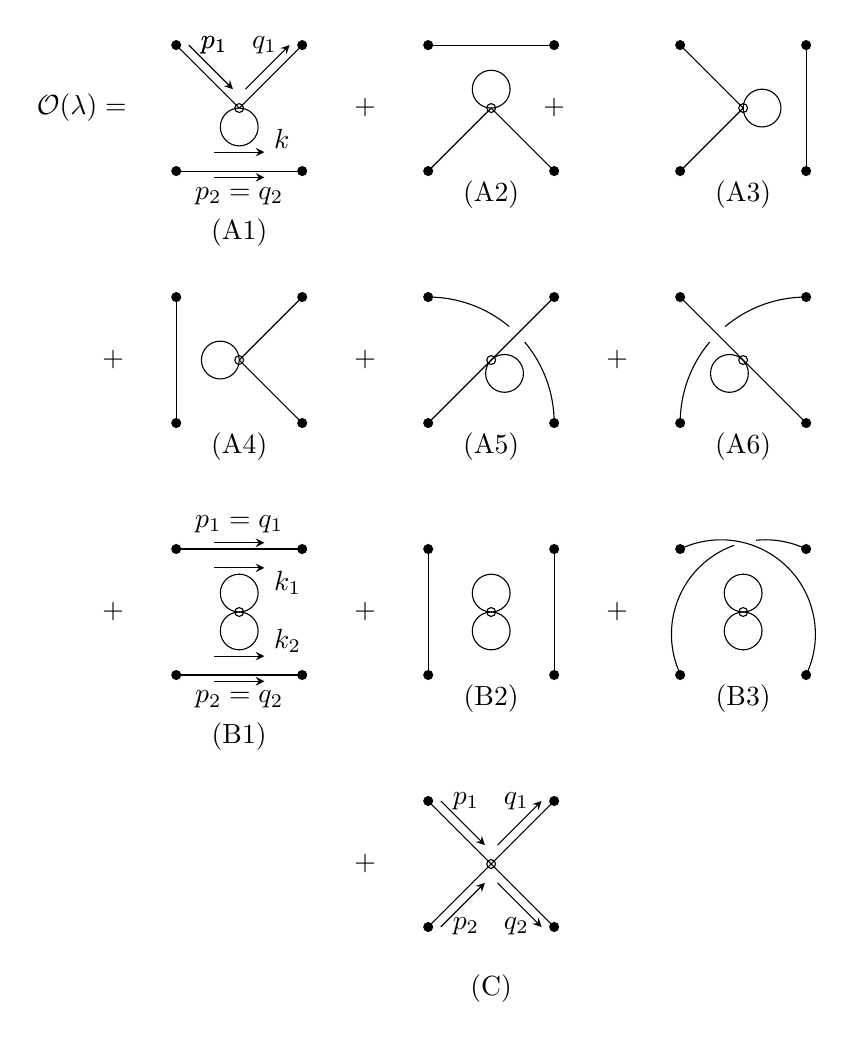
\begin{tikzpicture}[scale=0.8]
    \draw (-4.5,0) node {$\mathcal{O}(\lambda)=$};
    \filldraw (-3,1) circle (2pt);
    \filldraw (-1,1) circle (2pt);
    \filldraw (-1,-1) circle (2pt);
    \filldraw (-3,-1) circle (2pt);
    \draw (-2,0) circle (2pt);
    \draw (-2, -1.6) node[anchor=north] {(A1)};
    \draw (-3,1) -- (-2,0);
    \draw (-1,1) -- (-2,0);
    \draw (-1,-1) -- (-3,-1);
    \draw (-2, -0.3) circle (0.3);
    \draw[-stealth] (-2.8,1) -- (-2.1,0.3);
    \draw[stealth-] (-1.2,1) -- (-1.9,0.3);
    \draw (-1.6,0.7) node[anchor=south] {$q_1$};
    \draw (-2.4,0.7) node[anchor=south] {$p_1$};
    \draw[-stealth] (-2.4,-1.1) -- (-1.6,-1.1);
    \draw (-2,-1.1) node[anchor=north] {$p_2=q_2$};
    \draw (-2.4,0.7) node[anchor=south] {$p_1$};
    \draw[-stealth] (-2.4,-0.7) -- (-1.6,-0.7);
    \draw (-1.6,-0.8) node[anchor=south west] {$k$};
    
    \draw (0,0) node {$+$};

    \filldraw (3,1) circle (2pt);
    \filldraw (1,1) circle (2pt);
    \filldraw (1,-1) circle (2pt);
    \filldraw (3,-1) circle (2pt);
    \draw (2,0) circle (2pt);
    \draw (2, -1) node[anchor=north] {(A2)};
    \draw (3,-1) -- (2,0);
    \draw (1,-1) -- (2,0);
    \draw (1,1) -- (3,1);
    \draw (2, 0.3) circle (0.3);

    \draw (3,0) node {$+$};

    \filldraw (7,1) circle (2pt);
    \filldraw (5,1) circle (2pt);
    \filldraw (5,-1) circle (2pt);
    \filldraw (7,-1) circle (2pt);
    \draw (6,0) circle (2pt);
    \draw (6, -1) node[anchor=north] {(A3)};
    \draw (5,-1) -- (6,0);
    \draw (5,1) -- (6,0);
    \draw (7,1) -- (7,-1);
    \draw (6.3, 0) circle (0.3);

    \draw (-4,-4) node {$+$};

    \filldraw (-3,-3) circle (2pt);
    \filldraw (-1,-3) circle (2pt);
    \filldraw (-1,-5) circle (2pt);
    \filldraw (-3,-5) circle (2pt);
    \draw (-2,-4) circle (2pt);
    \draw (-2, -5) node[anchor=north] {(A4)};
    \draw (-1,-5) -- (-2,-4);
    \draw (-1,-3) -- (-2,-4);
    \draw (-3,-3) -- (-3,-5);
    \draw (-2.3, -4) circle (0.3);

    \draw (0,-4) node {$+$};

    \filldraw (1,-3) circle (2pt);
    \filldraw (3,-3) circle (2pt);
    \filldraw (3,-5) circle (2pt);
    \filldraw (1,-5) circle (2pt);
    \draw (2,-4) circle (2pt);
    \draw (2, -5) node[anchor=north] {(A5)};
    \draw (3,-3) -- (1,-5);
    \draw (2.212, -4.212) circle (0.3);
    \draw (3,-5) arc (0:40:2);
    \draw (2.28557521937,-3.46791111376) arc (50:90:2);

    \draw (4,-4) node {$+$};

    \filldraw (5,-3) circle (2pt);
    \filldraw (7,-3) circle (2pt);
    \filldraw (7,-5) circle (2pt);
    \filldraw (5,-5) circle (2pt);
    \draw (6,-4) circle (2pt);
    \draw (6, -5) node[anchor=north] {(A6)};
    \draw (5,-3) -- (7,-5);
    \draw (5.782, -4.212) circle (0.3);
    \draw (7,-3) arc (90:130:2);
    \draw (5.46791111376,-3.71442478063) arc (140:180:2);

    \draw (-4,-8) node {$+$};

    \filldraw (-3,-7) circle (2pt);
    \filldraw (-1,-7) circle (2pt);
    \filldraw (-1,-9) circle (2pt);
    \filldraw (-3,-9) circle (2pt);
    \draw (-2,-8) circle (2pt);
    \draw (-2, -9.6) node[anchor=north] {(B1)};
    \draw (-1,-7) -- (-3,-7);
    \draw (-1,-9) -- (-3,-9);
    \draw (-2, -8.3) circle (0.3);
    \draw (-2, -7.7) circle (0.3);
    \draw[-stealth] (-2.4, -6.9) -- (-1.6, -6.9);
    \draw[-stealth] (-2.4, -7.3) -- (-1.6, -7.3);
    \draw[-stealth] (-2.4, -8.7) -- (-1.6, -8.7);
    \draw[-stealth] (-2.4, -9.1) -- (-1.6, -9.1);
    \draw (-2,-6.9) node[anchor=south] {$p_1=q_1$};
    \draw (-1.6,-7.2) node[anchor=north west] {$k_1$};
    \draw (-1.6,-8.8) node[anchor=south west] {$k_2$};
    \draw (-2,-9.1) node[anchor=north] {$p_2=q_2$};

    \draw (0,-8) node {$+$};

    \filldraw (3,-7) circle (2pt);
    \filldraw (1,-7) circle (2pt);
    \filldraw (1,-9) circle (2pt);
    \filldraw (3,-9) circle (2pt);
    \draw (2,-8) circle (2pt);
    \draw (2, -9) node[anchor=north] {(B2)};
    \draw (1,-7) -- (1,-9);
    \draw (3,-7) -- (3,-9);
    \draw (2, -8.3) circle (0.3);
    \draw (2, -7.7) circle (0.3);

    \draw (4,-8) node {$+$};

    \filldraw (7,-7) circle (2pt);
    \filldraw (5,-7) circle (2pt);
    \filldraw (5,-9) circle (2pt);
    \filldraw (7,-9) circle (2pt);
    \draw (6,-8) circle (2pt);
    \draw (6, -9) node[anchor=north] {(B3)};
    \draw (6, -8.3) circle (0.3);
    \draw (6, -7.7) circle (0.3);
    \draw (7, -9) arc (-25.5287793655:115.528779366:1.5);
    \draw (7, -7) arc (64.4712206345:95.633022225:1.5);
    \draw (5.85754508895, -6.94075745063) arc (109.633022225:205.528779366:1.5);

    \draw (0,-12) node {$+$};

    \filldraw (1,-11) circle (2pt);
    \filldraw (3,-11) circle (2pt);
    \filldraw (3,-13) circle (2pt);
    \filldraw (1,-13) circle (2pt);
    \draw (2,-12) circle (2pt);
    \draw (2, -13.6) node[anchor=north] {(C)};
    \draw (3,-11) -- (1,-13);
    \draw (3,-13) -- (1,-11);
    \draw[stealth-] (2.8,-11) -- (2.1,-11.7);
    \draw[-stealth] (1.2,-11) -- (1.9,-11.7);
    \draw[stealth-] (2.8,-13) -- (2.1,-12.3);
    \draw[-stealth] (1.2,-13) -- (1.9,-12.3);
    \draw (1.6,-11.3) node[anchor=south] {$p_1$};
    \draw (2.4,-11.3) node[anchor=south] {$q_1$};
    \draw (1.6,-12.7) node[anchor=north] {$p_2$};
    \draw (2.4,-12.7) node[anchor=north] {$q_2$};

  \end{tikzpicture}
  \caption{Feynman diagrams for a $4$PCF $\braket{\hat \phi(p_1)\hat \phi(p_2) \hat \phi(q_1) \hat \phi(q_2)}$ in the interacting scalar theory. Each line is a Wick pair and each vertex is a point in spacetime.}
  \label{fig:feynman-construction}
\end{figure}

For a 4PCF in the scalar interacting theory there are four external vertices. There is one internal vertex to first order in $\lambda$. Following the rules for drawing edges, there are ten ways of pairing the $\phi$s to evaluate the numerator of (\ref{eqn:interacting-scalar-partway}) which are shown in Figure \ref{fig:feynman-construction}. Diagrams A1-A6 are similar, as are B1-B3, so we will only calculate one diagram from each of these classes. For this reason, only the momenta of this diagram are labeled. The direction in which momentum is chosen to flow is a matter of preference.

To calculate the 4PCF $\braket{\hat \phi(p_1)\hat \phi(p_2) \hat \phi(q_1) \hat \phi(q_2)}$ from a diagram, we follow (\ref{eqn:scalar-theory-npcf}) by writing $G(k)$ for every propagator with momentum $k$. For internal vertices, (\ref{eqn:momentum-conservation-at-vertex}) tells us to enforce momentum conservation by integrating over all momenta subject to the constraint that the total momentum of all the propagators connected to an internal vertex is zero. Thus diagram A1 diagrams evaluates to 
\begin{es}
  \mathrm{(A1)} &\propto G(p_1) G(q_1)G(p_2)\delta(p_2-q_2) \int \ftve{4}{k} \delta(p_1 - q_1 + k - k)G(k)\\
   &\propto G(p_1) G(q_1) \delta(p_1 - q_1)\delta(p_2-q_2)\int \ftve{4}{k} G(k).\\
  \label{eqn:scattering-diagram-a}
\end{es}
The proportionality statements acknowledge that we are focusing on the structure of the Green's functions and have not yet put in the correct powers of $\lambda$ or other coefficients that might appear.

The first delta function in line 1 is the delta function of (\ref{eqn:scalar-theory-npcf}), enforcing that momentum does not change along a propagator. The second delta function is the delta function of  (\ref{eqn:momentum-conservation-at-vertex}), enforcing that momentum cannot change at a vertex. For this diagram, these constraints together enforce that momentum of each must be conserved, and the double $\delta$-function in the above equation falls out to prevent the momenta from being mixed. That is, the free theory did not lead to momentum mixing in this case. It only changed the value of the 4PCF by some value $\int \ftve{4}{k} G(k)$ which we have not computed yet.

We can compute the diagrams (B1) and (C) in a similar way:
\begin{es}
  \mathrm{(B1)} &\propto G(p_1)\delta(p_1-q_1) G(p_2)\delta(p_2-q_2)\int \ftve{4}{k_1}\ftve{4}{k_2}G(k_1)G(k_2)\\
  \mathrm{(C)} &\propto G(p_1)G(p_2)G(q_1)G(q_2)\delta(p_1+p_2+q_1+q_2).
  \label{eqn:scattering-diagrams-b-c}
\end{es}

Diagram (B1) is like A1 in that it conserves momentum for each pair of particles. However, Diagram (C) allows the much-heralded momentum mixing. Even if $p_1$, $p_2$, $q_1$, and $q_2$ are all different, (C) will be nonzero as long as the momenta sum to zero. This diagram (and only this diagram) is the leading order contribution to $\phi\phi\rightarrow\phi\phi$ scattering, and we will use it a great deal throughout the rest of this chapter.

We have now verified that this $\phi^4$ theory allows particles to interact. Before moving on to quantify this interaction by computing scattering cross sections, it's worth covering two more details. The first is to replace the above two proportionality statements with actual equations. The second is to work out the denominator of (\ref{eqn:interacting-scalar-partway}) and divide the sum of the (A), (B), and (C) diagrams by that to have a full equation for the interacting theory $n$PCF.

\subsection{Symmetry Factor and Feynman Rules}
All of the diagrams drawn in figure \ref{fig:feynman-construction} were first order, since they contained only one power of $S_1$ and therefore only one power of $\lambda$. If we had written the diagrams of order $\lambda^2$, they would have had two internal vertices (one for each $S_1$). Thus, every diagram should be multiplied by the constant $i\lambda$ for every internal vertex.

Another potential worry is the possibility of under-counting. $S_1$ contains four $\phi$s, which can each be contracted with another $\phi$ in the $n$PCF. Contracting with the first $\phi$ and contracting with the second represent different contractions and should be added individually. But this is not reflected in our Feynman diagram, where we draw a contraction with any one of the $\phi$s as a propagator running into the internal vertex and make no note of which $\phi$ it was contracted with. Another source of error enters when we compute second order diagrams: these involve two identical $S_1$ values connected in different ways to the exterior vertices. We should double each diagram to reflect the fact that the two $S_1$ values could be swapped without changing the diagram structure. There are more numerical factors we haven't taken care of as well, which are all represented in table \ref{tab:symmetry-factor}.

\begin{table}
  \centering
  \bgroup
  \small
  \def\arraystretch{3}
  \begin{tabular}{c|c}
    \hline \hline
    Contribution & Source\\ \hline
    $\displaystyle \frac{(-i\lambda)^n}{n!}$ & Taylor series expansion of $e^{-iS_1}$\\
    $\displaystyle \frac{1}{4!}$ & Definition of the interacting term in the Lagrangian\\
    $n!$ & The number of ways to swap internal vertices\\
    $\displaystyle \frac{1}{(\mathrm{identical\ vertices})!}$ & \makecell{In the above row, we should not have swapped \\vertices which were already identical in the diagram}\\
    $4!$ & \makecell{The number of ways to connect 4 $\phi$s to 4 incoming\\ propagators for each internal vertex}\\
    $\displaystyle \frac{1}{2^{\mathrm{reversible\ propagators}}}$ & \makecell{In the above row, we should not have \\swapped propagators that both came \\from and led to the same vertex}\\
    \hline \hline
  \end{tabular}
  \caption{Factors we should multiply each Feynman diagram by due to expansion coefficients, over- or under-counting, and other sources. Here, $n$ represents the number of internal vertices.}
  \egroup
  \label{tab:symmetry-factor}
\end{table}

To get the total correction to each diagram, we multiply every entry in the left hand column of table \ref{tab:symmetry-factor}. Most of the entries cancel, but to keep track of those that don't, we define the \emphi{symmetry factor}
\begin{e}
  S_f = (1+\mathrm{identical\ vertices})!(1+\mathrm{reversible\ propagators})!
  \label{eqn:symmetry-factor}
\end{e}
where identical vertices are internal vertices which are connected to the same vertices as each other, and reversible propagators are those that lead to and out of the same internal vertex.
in which case we should multiply each diagram by the factor $(-i\lambda)^n / S_f$.

As an example, in figure \ref{fig:feynman-construction}, all the A diagrams have symmetry factor 2 due to the reversible propagator with momentum $k$. The B diagrams have symmetry factor 4 because they have two reversible propagators, and the C diagram has symmetry factor 1 because there are no reversible propagators or identical vertices.

The definition of the symmetry factor allows us to write down the value of any diagram exactly by following the following rules, called the \emphi{Feynman rules}:
\begin{enumerate}
  \item The edge \raisebox{0.2em}{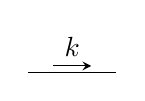
\begin{tikzpicture}[scale=0.8]
    \draw (-0.7,0) -- (0.7,0);
    \draw[-stealth] (-0.3,0.1) -- (0.3,0.1);
    \draw (-0,0.1) node[anchor=south]{$k$};
  \end{tikzpicture}} contributes $G(k)$
  \item A vertex \raisebox{-2.3em}{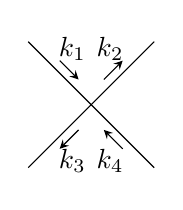
\begin{tikzpicture}[scale=0.8]
    \draw (-1,1) -- (1,-1);
    \draw (-1,-1) -- (1,1);
    \draw[-stealth] (-0.5,0.7) -- (-0.2,0.4);
    \draw (-0.3,0.55) node[anchor=south]{$k_1$};
    \draw[stealth-] (0.5,0.7) -- (0.2,0.4);
    \draw (0.3,0.55) node[anchor=south]{$k_2$};
    \draw[stealth-] (-0.5,-0.7) -- (-0.2,-0.4);
    \draw (-0.3,-0.55) node[anchor=north]{$k_3$};
    \draw[-stealth] (0.5,-0.7) -- (0.2,-0.4);
    \draw (0.3,-0.55) node[anchor=north]{$k_4$};
  \end{tikzpicture}} contributes $-i\lambda \delta(k_1 - k_2 - k_3 + k_4)$
  \item Every internal propagator $k$ is integrated over $\int \ftve{4}{k}$
  \item Diagrams with exchangeable vertices or reversible edges contribute a symmetry factor $S_f$.
\end{enumerate}

Once the diagrams are computed, they may be added and the sum divided by the denominator of (\ref{eqn:interacting-scalar-partway}), discussed in the next section, to get the $n$PCF

% \begin{figure}
%   \centering
%   \begin{tikzpicture}[scale=0.8]
%     \draw (-6.8,0) node {$\mathcal{O}(\lambda^2)=$};
%     \draw[black] (-5,0) node[anchor=east] {$x_1$};
%     \draw[black] (-3,0) node[anchor=west] {$x_2$};
%     \draw (-5,0) -- (-3,0);
%     \draw[black] (-3.7,-0.3) circle (0.3);
%     \draw[black] (-4.3,0.3) circle (0.3);

%     \draw (-2,0) node {$+$};

%     \draw[black] (-1,0) node[anchor=east] {$x_1$};
%     \draw[black] (1,0) node[anchor=west] {$x_2$};
%     \draw (-1,0) -- (1,0);
%     \draw[black] (0,-0.3) circle (0.3);
%     \draw[black] (0,-0.9) circle (0.3);
    
%     \draw (2,0) node {$+$};

%     \draw[black] (3,0) node[anchor=east] {$x_1$};
%     \draw[black] (5,0) node[anchor=west] {$x_2$};
%     \draw[black] (4,0) circle (0.5);
%     \draw (3,0) -- (5,0);

%     \draw (-6,-3) node {$+$};

%     \draw[black] (-5,-3) node[anchor=east] {$x_1$};
%     \draw[black] (-3,-3) node[anchor=west] {$x_2$};
%     \draw[black] (-3.6,-3) circle (0.3);
%     \draw[black] (-3.6,-3.6) circle (0.3);
%     \draw[black] (-4.4,-3) circle (0.3);
%     \draw[black] (-4.4,-3.6) circle (0.3);
%     \draw (-5,-3) arc (165:15:1.05);
   
%     \draw (-2,-3) node {$+$};

%     \draw[black] (-1,-3) node[anchor=east] {$x_1$};
%     \draw[black] (1,-3) node[anchor=west] {$x_2$};
%     \draw[black] (-0.6,-3.4) circle (0.3);
%     \draw[black] (-0,-3.4) circle (0.3);
%     \draw[black] (0.6,-3.4) circle (0.3);
%     \draw (-1,-3) arc (165:15:1.05);

%     \draw (2,-3) node {$+$};

%     \draw[black] (3,-3) node[anchor=east] {$x_1$};
%     \draw[black] (5,-3) node[anchor=west] {$x_2$};
%     \draw[black] (4,-3.4) circle (0.5);
%     \draw[black] (3.5,-3.4) -- (4.5, -3.4);
%     \draw (3,-3) arc (165:15:1.05);

%     \draw (-2,-6) node {$+$};

%     \draw[black] (-1,-6) node[anchor=east] {$x_1$};
%     \draw[black] (1,-6) node[anchor=west] {$x_2$};
%     \draw[black] (-0.3,-6.4) circle (0.3);
%     \draw[black] (0.3,-6.4) circle (0.3);
%     \draw[black] (0,-5.53) circle (0.3);
%     \draw (-1,-6) arc (165:15:1.05);
%   \end{tikzpicture}
%   \caption{Second order Feynman diagrams for the $\phi^4$ theory.}
%   \label{fig:feynman-second-order}
% \end{figure}


\subsection{The Denominator: Vacuum Diagram Cancellation}
This section deals with the denominator of (\ref{eqn:interacting-scalar-partway}):
$$\int \mathcal{D}\phi e^{-i S_0}e^{-iS_1}$$
which we must divide the sum of all Feynman diagrams by to get an $n$PCF. This factor came from requiring the $n$PCF to be normalized. Fortunately, this integral will cancel perfectly with terms in the numerator.

To see how, consider the diagrammatic expansion of this denominator. It is essentially a 0PCF, if such a thing exists. For scalar field theory, the zeroth order term is 1 and the the first order diagram is
\begin{center}
  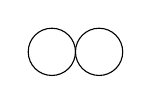
\begin{tikzpicture}
    \draw (-0.3,0) circle(0.3);
    \draw (0.3,0) circle(0.3);
  \end{tikzpicture}
\end{center}
where we have left out the circle to indicate the internal vertex (this is often done since any intersection of propagators is clearly a vertex).

This kind of diagram which is unconnected to external vertices called a \emphi{vacuum diagram}. You may recognize it diagram as a part of all the (B) diagrams in figure \ref{fig:feynman-construction}. In fact, the vacuum diagrams in the denominator will cancel with all of the diagrams in the numerator like (B) that have vacuum sub-diagrams. The mathematical explanation for this fact is that for every diagram like (A) or (C) that has no vacuum sub-diagrams, you can just multiply by a vacuum sub-diagram to get a diagram like (B), where both are combined. The reverse of this statement is that to divide by the vacuum diagrams, we need to remove all the diagrams like (B) that have vacuum sub-diagrams.

There is also physical intuition for removing by diagrams like (B) that have vacuum sub-diagrams. The vacuum diagrams have no external vertices, and external vertices generally represent particles. Thus, vacuum diagrams represent some change in energy of the vacuum, hence the name. Changes to the vacuum energy are generally undetectable, since we can only measure energy differences between systems and the vacuum is always present. For this reason, we should not count diagrams like (B) that measure the energy of the vacuum.\footnote{This is fortunate for us, since the vacuum diagrams can be infinite. The internal vertices come with integrals over momenta due to the Feynman rules, but the lack of external vertices gives fewer delta functions. For many internal vertices, the diagrams can blow up.}

Now that we know not to draw diagrams with vacuum sub-diagrams, we can fully compute any $n$PCF in the interacting theory with the Feynman rules. Our first and primary application for this newfound power will be to compute scattering amplitudes, which the next section is devoted to.

\section{Spin Zero Scattering}
\label{sec:spin-zero-scattering}
In this section, we'll compute scattering amplitudes for $\phi\phi \rightarrow \phi\phi$ and $\phi \rightarrow \phi\phi\phi$ to get used to $\phi^4$ theory and to practice with the Feynman rules. We'll follow up with a theory of two scalar particles and compute the probability of decay between the two.

Chapter \ref{chap:scattering} informed us that the scattering probability is the square of the $S$ matrix, where the $S$ matrix entry for $m$ particles with momenta $p_i$ scattering to $n$ particles with momenta $-q_i$is given by the $(m+n)$PCF for momenta $p_i$ and $q_i$. We noted however that the $S$ matrix is mostly zero; only when the incoming total momentum equals the outgoing momentum can scattering occur. This appeared in our calculation in the previous section of the 4PCF as well: every diagram in (\ref{eqn:scattering-diagram-a}) and (\ref{eqn:scattering-diagrams-b-c}) was multiplied by $\delta(p_1 + p_2 + q_1 + q_2)$.

We stripped off this delta function part by defining the scattering amplitude $-iM$ as the part of the $S$ matrix with $p_1 + p_2 + q_1 + q_2=0$, but excluding the no-scattering, diagonal entries where $p_1 = p_2$ and $q_1 = q_2$. The (A) diagrams for the 4PCF shown in figure \ref{fig:feynman-construction} had delta functions $\delta(p_1 - p_2)$ and $\delta(q_1-q_2)$, revealing these to be no-scattering diagrams. The only diagram that represents actual $\phi\phi\rightarrow\phi\phi$ scattering to first order is diagram C.

To extract a scattering amplitude from $C$, we must divide the corresponding $n$PCF by the propagator for each incoming and outgoing field, as \jtd{Equation number} dictates. The motivation for this was that we are not interested in the way the particles move before or after they interact, which is represented by the propagators connected to the external legs. We are interested in the actual interaction, which occurs in the middle of diagram (C). Once this division is complete, we get our first ever scattering amplitude:
\begin{e}
  -iM_{\phi\phi \rightarrow \phi \phi} = -i\lambda + \mathcal{O}(\lambda^2).
\end{e}
This equation is very simple, perhaps disappointingly so. Let's calculate the second-order contributions to the scattering amplitude to see if they are more interesting.

The first step is to draw new second-order diagrams. Many of these diagrams will look like this:
\begin{center}
  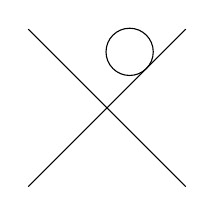
\begin{tikzpicture}
    \draw (-1,1)--(1,-1);
    \draw (-1,-1)--(1,1);
    \draw (0.28786796564, 0.71213203435) circle (0.3);
  \end{tikzpicture}
\end{center}
but these diagrams actually do not contribute to the scattering amplitude. Recall that the point of dividing by $G(p)$ for every external propagator $p$ was to account for the motion of a particle before it interacts. The loop in the above diagram represents particle activity after it has interacted with the rest of the diagram. This loop represents self-interaction and is interesting in its own right. In fact, we'll study it in section \ref{sec:scalar-mass}. However, it still represents a particle propagating on its own and we must divide it out. Therefore, this diagram is just the same $-i\lambda$ first-order diagram we computed above.

This is an example of a generalized rule for calculating scattering amplitudes: the only diagrams that contribute to amplitudes are \emphi{truncated}. The definition of truncated is as follows:
\begin{center}
  \textit{In a truncated diagram, no internal propagators can be cut that sever exactly one external vertex from the diagram.}
\end{center}
An internal propagator is one that does not connect directly to an external vertex. The above diagram was not truncated because the propagator between the central vertex and the loop could have been cut, and this would have severed the upper right external vertex from the diagram. However, the following diagrams \textit{are} truncated, and do contribute to the matrix amplitude:
\begin{e}
  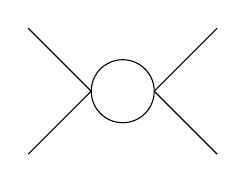
\begin{tikzpicture}[scale=0.8]
    \draw (-1,1)--(0,0);
    \draw (-1,-1)--(0,0);
    \draw (2,1)--(1,0);
    \draw (2,-1)--(1,0);
    \draw(0.5,0) circle (0.5);
  \end{tikzpicture}
  \qquad
  \raisebox{-1.1em}{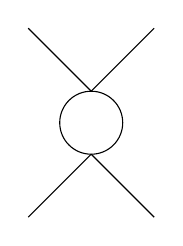
\begin{tikzpicture}[scale=0.8]
    \draw (1,-1)--(0,0);
    \draw (-1,-1)--(0,0);
    \draw (1,2)--(0,1);
    \draw (-1,2)--(0,1);
    \draw(0,0.5) circle (0.5);
  \end{tikzpicture}}
  \qquad
  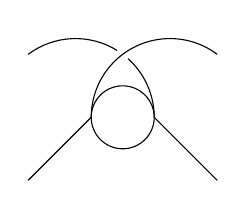
\begin{tikzpicture}[scale=0.8]
    \draw (-1,-1)--(0,0);
    \draw (2,-1)--(1,0);
    \draw (0.5,0) circle (0.5);
    \draw (2,1) arc (53.1301023542:180:1.25);
    \draw (1,0) arc (0:48.1301023542:1.25);
    \draw (0.40999028082,1.06156150515) arc (58.1301023542:126.869897646:1.25);
  \end{tikzpicture}.
  \label{eqn:scalar-second-order-2-2-diagrams}
\end{e}
\jtd{Put in momentum arrows}

These represent the first non-trivial effect of QFT we have seen. Everything we have done so far has confirmed classical expectations, from $M=\lambda$ above to momentum conservation. These diagrams are fundamentally quantum and relativistic phenomena and represent a a true prediction of QFT. Let's compute them using the Feynman rules. Two propagators in each diagram are identical and can be exchanged, so they have symmetry factors of 2. Thus,
\begin{es}
  \mathrm{Left} = -\frac{\lambda^2}{2}\int \ftve{4}{k} \frac{1}{k^2-m^2}\frac{1}{(k - p_1- p_2)^2-m^2}\\
  \mathrm{Center} = -\frac{\lambda^2}{2}\int \ftve{4}{k} \frac{1}{k^2-m^2}\frac{1}{(k - p_1- q_1)^2-m^2}\\
  \mathrm{Right} = -\frac{\lambda^2}{2}\int \ftve{4}{k} \frac{1}{k^2-m^2}\frac{1}{(k - p_1- q_2)^2-m^2}.
  \label{eqn:scalar-second-order-2-2-diagrams-values}
\end{es}
where we have removed the external propagators in the spirit of truncation. It's common to deal with these diagrams by defining \emphi{Mandelstam variables}, which are a reparametrization for any two-to-two-particle interaction:
\begin{e}
  s = (p_1 + p_2)^2\qquad t = (p_1 - q_1)^2 \qquad u = (p_1 - q_2)^2.
  \label{eqn:mandelstam}
\end{e}
There are three variables because momentum conservation makes a fourth one obsolete. They have the interpretation that $s$ is the incoming momentum, equivalently the energy in the center of mass frame, and $t$ and $u$ represent the amount of momentum transfer. Calculation will reveal that each diagram is sensitive only to $s$, $t$, or $u$ respectively, so all three diagrams can be added up as follows:
\begin{e}
  -iM = -i\lambda - \lambda^2\parens{V(s) + V(t) + V(u)} + \mathcal{O}(\lambda^3)
  \label{eqn:2-2-scalar-amplitude}
\end{e}
where
\begin{e}
  V(s) = \frac{1}{2}\int \ftve{4}{k} \frac{1}{k^2-m^2} \frac{1}{(k - p_1 - p_2)^2-m^2}.
  \label{eqn:2-2-scalar-v}
\end{e}
This integral may strike you as a bit peculiar. Let's pretend for a moment that $k^2$ is the Euclidean norm $k_0^2 + \bm k^2$ rather than the Minkowski norm $k_0^2 - \bm k^2$. Then we could switch to spherical coordinates and $d^4 k$ would become $k^3 dk$ times a radial volume element $d\Omega$. For large $k$, this $k^3$ cancels with the integrand, which goes like $k^{-4}$, leading to an overall trend of $\int^\infty dk /k$. This integral is divergent.

The techniques for handling this divergence took a great deal of time to be developed historically. They necessitate a change in thinking which we will discuss in chapter \ref{chap:renormalization}, so we'll postpone this particular integral until then. In three spacetime dimensions (two spatial dimensions), the integral trends to $\int^\infty dk /k^2$ which is a perfectly reasonable number. Figure \ref{fig:2-2-scalar-v-3d} shows the plot of $V(s)$ in three dimensions.\footnote{You might reasonably object to us computing predictions for an unphysical universe, like one with only three spacetime dimensions, in a book about the phenomena of this universe. However, many of the phenomena we'll see are qualitatively similar between dimensions, and the characteristics of dimension four specifically will be covered later.}

\begin{figure}
  \centering
  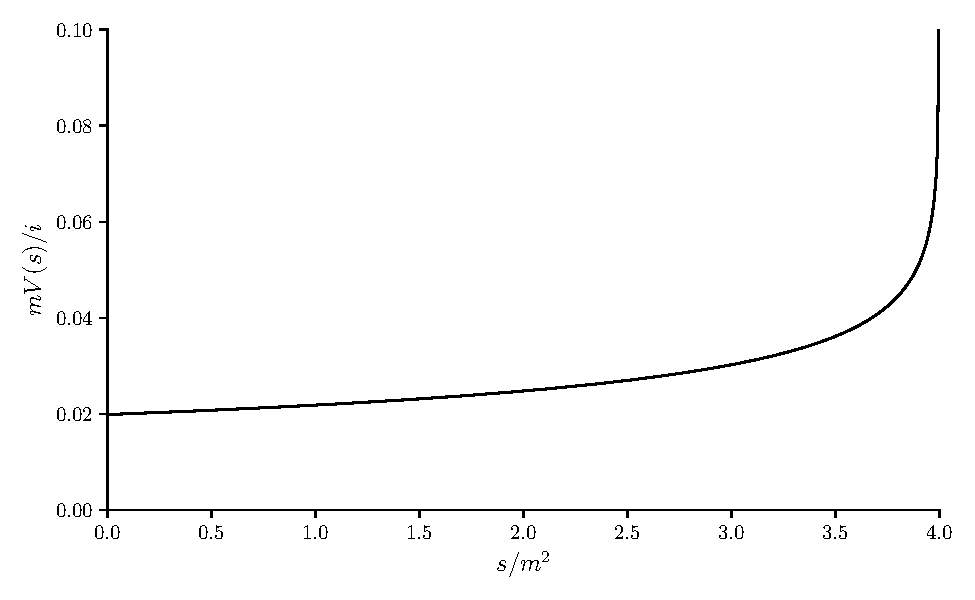
\includegraphics[width=\linewidth]{figs/2-2-scalar-v-3d.pdf}
  \caption{$mV(s)/i$, the unitless second order component of the scattering amplitude. This is computed for two scalar particles in 3 spacetime dimensions of center-of-mass energy $s$.}
  \label{fig:2-2-scalar-v-3d}
\end{figure}

Something immediately apparent about Figure \ref{fig:2-2-scalar-v-3d} is that the values are small. Multiplied by a small number $\lambda^2$ as \ref{eqn:2-2-scalar-amplitude} requires, and this $V(s)$ correction will be tiny except near the maximum value of $s=4m^2$, where the function blows up. This is the hyper-relativistic limit, where the particles are colliding at enormous speeds. In this limit, the quantum corrections introduced by the second-order diagrams can become arbitrarily large. (\ref{eqn:2-2-scalar-v}) is actually analytical computable:
\begin{e}
  V(s) = \frac{i}{16\pi \sqrt{s}}\ln \parens{\frac{m +\sqrt{s/4}}{m -\sqrt{s/4}}}.
\end{e}
We will discuss how to arrive at this value for the integral in chapter \ref{chap:renormalization}.

Taking the limit as $s\rightarrow 4$ reveals that $V(s)$ blows up and scattering becomes extremely intense. This is a QFT correction to the classical expectation that $M = \lambda$; i.e., scattering amplitude is independent of energy.

\subsection{Intuition for Feynman Diagrams}

In the derivation of this chapter, each propagator in a Feynman diagram represents a Wick contraction, but there is an intuitive picture for Feynman diagrams beyond the mathematical structure of Wick's theorem. We already know an external propagator --- a particle that links to an external vertex --- represents a particle entering the scattering experiment. Why not view \textit{every} propagator as a particle? Then the $\phi^4$ term of the Lagrangian, which corresponds to four propagators meeting at a vertex $x$ in a diagram, really does represent an interaction at $x$. A diagram with a loop, such as those in (\ref{eqn:scalar-second-order-2-2-diagrams}), represent two particles colliding, only for the outgoing particles to collide with each other again. If one collision is rare, then this secondary collision should be rarer than one collision only, which explains why these diagrams are small. On the other hand, if a collision is common, we might expect every particle pair to collide not just once or twice but many times, in which case we would have to draw infinitely many diagrams. It is at this point that QFT is no longer perturbative, and alternative methods to Feynman diagrams must be taken to compute scattering amplitudes.

There is a small problem with this picture, however. The two internal propagators in (\ref{eqn:scalar-second-order-2-2-diagrams}) are not real particles in a key sense: they are not on-shell. This can be seen in (\ref{eqn:scalar-second-order-2-2-diagrams-values}): we integrate $k$ over all four-dimensional space without requiring $k^2=m^2$. Instead, we call these internal propagators \emphi{virtual particles}, which interact like normal particles except that they can be off-shell (meaning that $k^2$ needn't equal $m^2$) and are never observed.

These virtual particles could have been predicted even before we saw the QFT principle of least action. One of the major results of special relativity was that mass is a form of energy, and a result of quantum mechanics is that a quantum particle may tunnel through a high-energy barrier in order to reach a low energy final state. Any theory of quantum mechanics and relativity, such as QFT, should combine these two well-understood phenomena. What better way to combine them than to allow particles to ``tunnel'' into an unphysical, perhaps higher-energy state before reaching a final state? The loop propagators represent this higher-energy state, and are unphysical in the same way that the electron should not classically exist in a high-energy barrier in quantum mechanics. Nevertheless, a particle can pass through the high-energy state in order to attain a different final state.

We could even have predicted that virtual particles can be off-shell by another example of hybrid quantum mechanical and relativistic reasoning: the energy-time uncertainty principle predicts that quantum states with a short lifetime have uncertain energies. In a relativistic context, the equivalent statement is that particles with a short lifetime have uncertain mass. Virtual particles are never observed, so they have effectively zero lifetime and infinitely uncertain mass, preventing the enforcement of the on-shell constraint.

We'll often treat any diagram with a loop, such as those of (\ref{eqn:scalar-second-order-2-2-diagrams}), as a ``quantum correction'' --- a small correction quantum mechanics imposes on a classical theory. The loop brings all the quantum effects mentioned in the previous paragraphs into the picture; it is comprised of virtual particles and the $\int d^4 k$ represents the fact that these virtual particles are off-shell. Figure \ref{fig:2-2-scalar-v-3d} for the second-order $\phi\phi \rightarrow \phi\phi$ amplitude was our first example of a quantum corrections, but more will appear such as mass, energy, magnetic and electric dipole moment corrections.

The diagrams without loops, often called \emphi{tree-level diagrams}, generally represent the properties of a classical theory that could be attained by merely minimizing the action via the Euler-Lagrange equations. For example, a tree-level diagram delivered us $M_{\phi\phi\rightarrow \phi\phi} = \lambda$ as classical thinking would suggest.


\section{Complex Scalar Theory}
So far, we've considered only real scalar fields where $\phi^* = \phi$, but one may well ask if complex scalar fields exist. After all, the fermions in Nature can all take on complex values, and the only fundamental scalar particle in Nature (the Higgs) is complex. Fortunately for us, generalizing the above results to a complex field will be mathematically easy. However, it will bring up a critical new physics concept which we will need to understand: the antiparticle.

\subsection{Antiparticles}

The Lagrangian of a complex scalar field is nearly the same as that of a real field. The only differences are coefficients to the term and the presence of complex conjugates:
\begin{e}
  \mathcal{L} = -|\del_\mu \phi|^2 - m^2 |\phi|^2 + \lambda |\phi|^4.
  \label{eqn:complex-scalar-lagrangian}
\end{e}
The reason why the coefficients have changed is so that the counting arguments of table \ref{tab:symmetry-factor} which allow computation of the symmetry factor still apply even though now $\phi^* \neq \phi$.

Immediately, we suspect that $\phi^*$ may be the antiparticle of $\phi$. This is because, as mentioned in chapter \ref{chap:intro}, an antiparticle is the mirror image of a particle under CPT (charge-parity-time) reversal symmetry. Parity and time reversal do nothing on this $\phi$ scalar particle, but charge reversal is manifested in complex conjugation \jtd{why?}, so that CPT symmetry takes $\phi$ to $\phi^*$. Thus, $\phi^*$ is the antiparticle of $\phi$.

The antiparticle explanation may not be fully satisfying, however, since (\ref{eqn:complex-scalar-lagrangian}) still looks like the Lagrangian of only one particle. Let's therefore break up the $\phi$ field into components. Just as a complex number $z=(a+ib)\sqrt{2}$ can be broken into two real components (the $\sqrt{2}$ is for normalization), the complex field $\phi = (\phi_a + i\phi_b)/\sqrt{2}$ can be broken into real fields $\phi_a$ and $\phi_b$. Plugging these into the Lagrangian, we get
\begin{es}
  \mathcal{L} =& -\frac{1}{2}(\del_\mu \phi_a)^2- \frac{m^2}{2} \phi_a^2 + \frac{\lambda}{4} \phi_a^4\\
  &-\frac{1}{2}(\del_\mu \phi_b)^2 - \frac{m^2}{2} \phi_b^2  + \frac{\lambda}{4} \phi_b^4\\
  &+ \frac{\lambda}{2}\phi_a^2 \phi_b^2.
  \label{eqn:complex-scalar-components}
\end{es}
We can now see that the complex scalar Lagrangian is just two real fields with the same mass $m$, same self-interaction $\lambda$, and an $a-b$ interaction term which is the last line. These properties were required for (\ref{eqn:complex-scalar-lagrangian}) to be written so simply.

The complex scalar Lagrangian (\ref{eqn:complex-scalar-lagrangian}) looks elegant, but when broken into its components it seems oddly contrived. Why should the real and imaginary parts have the same mass and interaction strengths? Why should they interact with each other in the exact way shown by (\ref{eqn:complex-scalar-components})? These constraints are imposed by CPT symmetry. A particle's antiparticle must have the same mass and interactions. Mathematically speaking, they obey a \emphi{symmetry}, in that swapping $\phi_a$ and $\phi_b$ does not change the Lagrangian.

In fact, the symmetry is even deeper than this; any (normalized) linear combination of the two fields is also indistinguishable from $\phi_a$ and $\phi_b$. For example, if we define $\chi_a = (3\phi_a + 4i\phi_b)/5$and $\chi_b = (4\phi_a - 3i\phi_b)/5$, we could rewrite (\ref{eqn:complex-scalar-components}) in terms of $\chi_a$ and $\chi_b$ and we would get the exact same form, just with $\phi$ swapped out for $\chi$. If it weren't for the odd $\frac{\lambda}{2}\phi_a^2\phi_b^2$ interaction term, this would not be true. \jtd{Unitary group too}

This particular symmetry is called SO(2), or \emphi{the Special Orthogonal Group of Order 2}. The name is motivated by the kinds of linear combinations which do not change the Lagrangian; ``special'' indicates that the new linear combinations $\chi$ must remain normalized, ``orthogonal'' indicates that the two fields $\chi_a$ and $\chi_b$ must have the same product as the original $\phi_a\phi_b$, ``group'' indicates that any linear combination that satisfies these two properties is allowed as a symmetry of the Lagrangian, and ``order 2'' means that the linear combination acts on two fields $\phi_a$ and $\phi_b$. This is our first example of a \emphi{continuous symmetry} because the set of available linear combinations is continuous. Nature adores continuous symmetries. The Standard Model which is the best known description of the fundamental particles has three of these symmetries, as will be discussed in the next part of this book.

You might wonder where $\phi$'s antiparticle was for the real scalar field case. For real scalars, the particle is its own antiparticle. This also occurs for some Standard Model particles, such as the photon.

\subsection{Feynman Rules for Complex Scalars}

Now that we have shown that a complex scalar contains an antiparticle, it is time to discuss the Feynman rules of the new theory. Fortunately, we do not have to repeat the many pages of derivations necessary for the real field theory. The Lagrangian is essentially the same, so the Green's function of a complex scalar field is identical to that of a real field. Wick's theorem and its application to the free theory and the interacting theory did not rely on anything other than that the perturbation $\lambda$ is small. Thus, we can skip straight to the rules for how to draw Feynman diagrams.

The new Lagrangian restricts diagrams slightly. The $\phi^4$ term became $\phi^*\phi \phi^*\phi$, meaning that only two antiparticles and two particles can meet at a vertex, not three and one, for instance. We'll have to enforce this in Feynman diagrams with a graphical rule. Suppose we draw an arrow on a propagator, where the arrow points one way for a particle and another way for an antiparticle. Then the $\phi^*\phi \phi^*\phi$ term means every vertex must have two arrows leading in and two leading out. (Since $\phi$ and $\overline \phi$ have opposite charge, you can think of these arrows as charge arrows.) Thus, the Feynman rules are 

\begin{enumerate}
  \item The edge \raisebox{0.2em}{\begin{tikzpicture}[scale=0.8]
    \draw (-0.7,0) -- (0.7,0);
    \draw[-{Latex[length=3mm]}] (-0.3,0) -- (0.15,0);
    \draw (-0,0.1) node[anchor=south]{$k$};
  \end{tikzpicture}} contributes $G(k)$
  \item A vertex \raisebox{-2.3em}{\begin{tikzpicture}[scale=0.8]
    \draw (-1,1) -- (1,-1);
    \draw (-1,-1) -- (1,1);
    \draw[-{Latex[length=3mm]}] (-0.5,0.5) -- (-0.2,0.2);
    \draw (-0.3,0.55) node[anchor=south]{$k_1$};
    \draw[{Latex[length=3mm]}-] (0.5,0.5) -- (0.2,0.2);
    \draw (0.3,0.55) node[anchor=south]{$k_2$};
    \draw[{Latex[length=3mm]}-] (-0.5,-0.5) -- (-0.2,-0.2);
    \draw (-0.3,-0.55) node[anchor=north]{$k_3$};
    \draw[-{Latex[length=3mm]}] (0.5,-0.5) -- (0.2,-0.2);
    \draw (0.3,-0.55) node[anchor=north]{$k_4$};
  \end{tikzpicture}} contributes $-i\lambda \delta(k_1 - k_2 - k_3 + k_4)$
  \item Every internal propagator $k$ is integrated over $\int \ftve{4}{k}$
  \item Diagrams with exchangeable vertices or reversible edges contribute a symmetry factor $S_f$.\footnote{You might recall that the definition of $S_f$ derived from a counting problem for how much each diagram should be weighted by, and that problem depended on $\phi$ being real. The coefficients of the new Lagrangian (\ref{eqn:complex-scalar-lagrangian}) have been carefully chosen so that the definition of the symmetry factor is the same, so we don't have to worry about redoing that argument.}
\end{enumerate}
We stopped drawing the momentum arrows in the diagrams to reverse clutter. There's no harm in just defining momentum to point in the same direction as the charge arrows.

As an example, here are the diagrams of (\ref{eqn:scalar-second-order-2-2-diagrams}) for a complex scalar field, representing $\phi \overline\phi \rightarrow \phi \overline\phi$ scattering:

\begin{e}
  \begin{tikzpicture}[scale=0.8]
    \draw (-1,1)--(0,0);
    \draw[-{Latex[length=2mm]}](-1,1)--(-0.5,0.5);
    \draw (-1,-1)--(0,0);
    \draw[{Latex[length=2mm]}-](-1,-1)--(-0.5,-0.5);
    \draw (2,1)--(1,0);
    \draw[{Latex[length=2mm]}-](2,1)--(1.5,0.5);
    \draw (2,-1)--(1,0);
    \draw[-{Latex[length=2mm]}](2,-1)--(1.5,-0.5);
    \draw(0.5,0) circle (0.5);
  \end{tikzpicture}
  \qquad
  \raisebox{-1.1em}{\begin{tikzpicture}[scale=0.8]
    \draw (1,-1)--(0,0);
    \draw[-{Latex[length=2mm]}](1,-1)--(0.5,-0.5);
    \draw (-1,-1)--(0,0);
    \draw[{Latex[length=2mm]}-](-1,-1)--(-0.5,-0.5);
    \draw (1,2)--(0,1);
    \draw[{Latex[length=2mm]}-](1,2)--(0.5,1.5);
    \draw (-1,2)--(0,1);
    \draw[-{Latex[length=2mm]}](-1,2)--(-0.5,1.5);
    \draw(0,0.5) circle (0.5);
  \end{tikzpicture}}
  \qquad
  \begin{tikzpicture}[scale=0.8]
    \draw (-1,-1)--(0,0);
    \draw[{Latex[length=2mm]}-](-1,-1)--(-0.5,-0.5);
    \draw (2,-1)--(1,0);
    \draw[-{Latex[length=2mm]}](2,-1)--(1.5,-0.5);
    \draw (0.5,0) circle (0.5);
    \draw (2,1) arc (53.1301023542:180:1.25);
    \draw[-{Latex[length=2mm]}](-0.4,1.25)--(-0.3,1.25);
    \draw[{Latex[length=2mm]}-](1.4,1.25)--(1.3,1.25);
    \draw (1,0) arc (0:48.1301023542:1.25);
    \draw (0.40999028082,1.06156150515) arc (58.1301023542:126.869897646:1.25);
    \draw[{Latex[length=2mm]}-](0.4,-0.5)--(0.5,-0.5);
    \draw[{Latex[length=2mm]}-](0.4,0.5)--(0.5,0.5);
  \end{tikzpicture}.
\end{e}

There are similar diagrams for $\phi\phi \rightarrow \phi \phi$ scattering:

\begin{e}
  \begin{tikzpicture}[scale=0.8]
    \draw (-1,1)--(0,0);
    \draw[-{Latex[length=2mm]}](-1,1)--(-0.5,0.5);
    \draw (-1,-1)--(0,0);
    \draw[-{Latex[length=2mm]}](-1,-1)--(-0.5,-0.5);
    \draw (2,1)--(1,0);
    \draw[{Latex[length=2mm]}-](2,1)--(1.5,0.5);
    \draw (2,-1)--(1,0);
    \draw[{Latex[length=2mm]}-](2,-1)--(1.5,-0.5);
    \draw(0.5,0) circle (0.5);
    \draw[-{Latex[length=2mm]}](0.4,-0.5)--(0.5,-0.5);
    \draw[-{Latex[length=2mm]}](0.4,0.5)--(0.5,0.5);
  \end{tikzpicture}
  \qquad
  \raisebox{-1.1em}{\begin{tikzpicture}[scale=0.8]
    \draw (1,-1)--(0,0);
    \draw[{Latex[length=2mm]}-](1,-1)--(0.5,-0.5);
    \draw (-1,-1)--(0,0);
    \draw[-{Latex[length=2mm]}](-1,-1)--(-0.5,-0.5);
    \draw (1,2)--(0,1);
    \draw[{Latex[length=2mm]}-](1,2)--(0.5,1.5);
    \draw (-1,2)--(0,1);
    \draw[-{Latex[length=2mm]}](-1,2)--(-0.5,1.5);
    \draw(0,0.5) circle (0.5);
  \end{tikzpicture}}
  \qquad
  \begin{tikzpicture}[scale=0.8]
    \draw (-1,-1)--(0,0);
    \draw[-{Latex[length=2mm]}](-1,-1)--(-0.5,-0.5);
    \draw (2,-1)--(1,0);
    \draw[{Latex[length=2mm]}-](2,-1)--(1.5,-0.5);
    \draw (0.5,0) circle (0.5);
    \draw (2,1) arc (53.1301023542:180:1.25);
    \draw[-{Latex[length=2mm]}](-0.4,1.25)--(-0.3,1.25);
    \draw[{Latex[length=2mm]}-](1.4,1.25)--(1.3,1.25);
    \draw (1,0) arc (0:48.1301023542:1.25);
    \draw (0.40999028082,1.06156150515) arc (58.1301023542:126.869897646:1.25);
  \end{tikzpicture}.
\end{e}
When a loop is drawn without charge arrows, the charge arrows can go either way so long as they are antiparallel. This does \textit{not} count as a reversible edge in the symmetry factor sense; a symmetry factor represents that we have overcounted a diagram, whereas if a loop can run either of two directions we are undercounting the diagrams. Thus, we should double each diagram where the loop can run either day, not half it.

Thus, a difference between complex scalar scattering and real scalar scattering is that the quantum corrections to complex scattering is more intense. Contributions from both particles and antiparticles can occur, increasing the total interaction strength. The exception is in some channels which forbid particle-antiparticle interactions. For example, for $\phi \phi \rightarrow \phi\phi$, the $s$ channel is not amplified because only $\phi$ particles may mediate that interaction. In $\phi \overline\phi \rightarrow \phi\overline\phi$, the $u$ channel is not amplified.

One of the most famous properties of matter and antimatter is that they explode on contact with each other. Electrons and positrons annihilate to two or three photons, as do neutral pions. Charged pions decay to muons and neutrinos, et cetera. In the next section,  we'll introduce a real scalar field as a photon-like particle and compute amplitudes for a complex scalar field to decay in this theory.

\section{Scalar Decay}
Let's create a theory with two particles: a complex scalar $\phi$ and a real scalar $\chi$ and an interaction between them of $\phi \phi^* \chi$. This corresponds to a Lagrangian of
\begin{e}
  \mathcal{L} = -|\del_\mu \phi|^2 - m_\phi|\phi|^2 - \frac{1}{2}(\del_\mu \chi)^2 - \frac{1}{2}m_\chi\chi^2 - g \phi\phi^* \chi.
\end{e}
In order to draw Feynman diagrams for a system with two particles, we need two types of lines --- a dashed line for $\chi$ and a solid line for $\phi$. The Feynman rules are as you might guess; the $\phi$ and $\chi$ propagators are still $G(k)$, momentum conservation is still applied at every vertex, and internal propagators are still integrated over. The only difference comes from the new interaction terms, which allows vertices connecting two $\phi$ particles to one $\chi$ particle
\begin{center}
  \feynmandiagram [horizontal=b to a, scale=0.8] {
    i1 -- [fermion] b -- [fermion] i2,
    a -- [scalar] b,
  };
\end{center}
which contributes an amplitude of $-ig$. Note that there is no charge arrow on the dashed $\chi$ line because $\chi$ is real and therefore uncharged.

Many interesting phenomena can be studied in this theory, but in this section we will only focus on one: the decay of $\chi$ into two $\phi$ particles. Due to energy conservation, this decay can only occur if $m_\chi > 2m_\phi$, so we assume this inequality.

The leading order interaction for decay is just the above Feynman diagram with some added labels
\begin{center}
  \feynmandiagram [vertical=b to a, scale=0.8] {
    i1 -- [fermion, momentum=$q$] b -- [fermion, momentum=$q$] i2,
    a -- [scalar, momentum=$0$] b,
  };
\end{center}
We've also rotated the diagram because, when drawing diagrams for scattering experiments, it is traditional to put the initial state at the bottom and the final state at the top so that time flows upwards as in embedding diagrams in relativity. We assumed that the $\chi$ particle is at rest, which we can always undo by boosting into a different reference frame if needed. The only truncated next order diagram is
\begin{center}
  \feynmandiagram [vertical=b to a, scale=0.8] {
    i1 -- [fermion] p1 -- [fermion, momentum=$q-k$] b -- [fermion, momentum=$q-k$] p2 -- [fermion] i2,
    a -- [scalar] b,
    p1 -- [scalar, momentum'=$k$] p2,
  };
\end{center}
Together, these diagrams produce a decay amplitude of 
\begin{e}
  iM = -ig + (-ig)^3\int \ftve{4}{k} \frac{1}{k^2-m_\chi^2}\frac{1}{[(q-k)^2-m_\phi^2]^2}
\end{e}
which yields a decay rate given by (\ref{eqn:total-decay-rate}). For the rest of this discussion, we'll neglect the second order term and just use $M=-g$.

Energy conservation gives $2q^0 = m_\chi$ and the on-shell constraint dictates that $(q^0)^2 - \bm q^2 = m_\phi^2$, so the momentum of the outgoing particles is $\bm q^2 = m_\phi^2 - m_\chi^2 / 4$. Thus, the three-dimensional integral over outgoing momenta is actually a two-dimensional integral on a sphere, and the spherical symmetry of this decay problem implies that the value is $4\pi$ times the integrand. Thus,
\begin{e}
  \Gamma = \frac{|M_{p\rightarrow q}|^2}{(2\pi)^5 m_\chi^3}\parens{m_\phi^2 - \frac{m_\chi^2}{4}}
\end{e}
It's more interesting to compute the unitless constant $\Gamma m_\chi^2$ --- physically, the probability to decay within one Compton wavelength of the particle, as a function of the ratio of $\mu = 2m_\phi / m_\chi < 1$. This is
\begin{e}
  m_\chi \Gamma = \frac{1-\mu^2}{4(2\pi)^5}g^2
\end{e}

One can see that as the decay products get lighter and $\mu$ gets smaller, the lifetime of $\chi$ becomes shorter. This is intuitively what we expect of our first every decay width calculation. Decay is the relativistic version of quantum tunneling into a new state, and quantum tunneling is generally more likely to happen if the potential energy of the end state is lower. Here, the mass energy of the end state is proportional to $\mu$, so we expect the lifetime to decrease with $\mu$. 

Another intuitive fact is that, for $\mu = 0$, $\Gamma$ reaches a finite value. This is something we should have expected because many particles in Nature, such as the pion, decay into massless photons. Yet the neutral pion has a relatively long lifetime of seconds, corresponding to a travel distance of 25 nanometers when moving at the speed of light (many particles live even shorter lives). Ignoring the fact that photons are not complex scalar particles, it would be concerning if our current calculations predicted zero lifetime for such decays.

If $m_\chi < m_\phi$, this decay is energetically forbidden, and completely new physics arises from the same Lagrangian which is discussed in the next section.

\section{Coulomb Potential for Scalars}
\label{sec:scalar-coulomb}
One of the foundational assumptions of QFT was that the theory is local, meaning that every particle is influenced only by its immediate environment. This might seem obviously incorrect at first because of long-range forces like Coulomb's law, which allow distant objects to affect one another. But in electromagnetism we explained these forces via a field which propagates information between objects by the means of waves, and in QFT we graduate those waves to particles. In this section we use the same Lagrangian as in the previous to demonstrate a long-range force carrier.

As an experiment to look for forces, we could scatter a complex scalar $\phi$ particle off of an equally charged $\phi$ particle and measure the cross section. The light, real scalar $\chi$ will carry the force between the two particles. The leading order diagram for this interaction is
\begin{center}
  \feynmandiagram [horizontal=b to a] {
    i1 -- [fermion, momentum'=$p_1$] b -- [fermion, momentum'=$q_1$] i2,
    j1 -- [fermion, momentum=$p_2$] a -- [fermion, momentum=$q_2$] j2,
    b -- [scalar, momentum=$p_1 - q_1$] a,
  };
\end{center}
If the outgoing particles were distinguishable then there would be a second diagram wherein the particles are swapped, but in this case the outgoing particles are equally charged and are indistinguishable. Setting $m_\chi=0$, the scattering amplitude is
\begin{e}
  iM = \frac{-ig^2}{(p_1 - q_1)^2}
\end{e}
which is just a constant times the Green's function for the one internal propagator.

We can use this scattering amplitude to compute the equivalent of the potential between the particles if we make a few approximations. Firstly, we'll work in the non-relativistic limit, where the energies of all particles is approximately their masses, in which case $p_1 - q_1$ has zero temporal component. The second approximation is to compare this amplitude with that predicted by non-relativistic quantum mechanics under the Born approximation, as discussed in appendix \ref{app:quantum}. That amplitude is $M(\bm p_1 - \bm q_1) = -V(\bm p_1 - \bm q_1)$ where $V$ is the Fourier transform of the potential between particles. Plugging in our amplitude calculation, we have
\begin{e}
  V(\bm x) = -g^2\int \ftve{3}{\bm \ell}\frac{e^{i\bm \ell \cdot \bm x}}{\bm \ell^2}
\end{e}
where $\bm \ell = \bm p_1 - \bm p_2$. By inspection, the integral cannot depend on the orientation of $\bm x$, so we write $\bm x = r \hat{\bm z}$ and switch to spherical coordinates:
\begin{es}
  V(r) &= -\frac{g^2}{4\pi^2} \int_{-1}^1 d\cos\theta \, \int_0^\infty d\ell \, e^{i\ell r \cos \theta}\\
  &= -\frac{g^2}{8\pi^2}\int_{-1}^1 d\cos\theta \, \int_{-\infty}^\infty d\ell \, e^{i\ell r \cos \theta}\\
  &= -\frac{g^2}{4\pi}\int_{-1}^1 d\cos\theta \, \delta(r \cos \theta)\\
  &= -\frac{g^2}{4\pi r}\\
\end{es}
The second line came about by recognizing that the real part of the integrand was symmetric under $\ell \rightarrow -\ell$, so we could extend the $\ell$ integral. The third line applied the theorem connecting the integral of an oscillating exponent to the delta function. The last line came from the fact that $\delta(f(x)) = \delta(x)/f'(x)$.

If we interpret the $g$ as the ``charge'' of the scalar particle, then the result is the Coulomb potential! In case the QFT principle of least action were still in doubt, this is an excellent sign that the theory is pointing us in the right direction. The only strangeness is that the sign is wrong; these like-charged particles are attracted to each other whereas in electromagnetism they would be repelled. This is a result of our choice to use scalar particles. In the next two chapters we will introduce new particles which are capable of flipping this sign to become more electromagnetism-like.

Another motivation for us to pursue more particles to describe electromagnetism is that this theory contains no magnetic field. There aren't enough degrees of freedom in the particles provided to store the direction of an additional field, and adding new ``magnetic field particles'' would not be able to interact so as to guarantee Maxwell's equations. We will need a particle capable of encoding the direction of the magnetic field within its quantum state.


\section{Massless Scalars are Rare}
\label{sec:scalar-mass}
One final problem with the Coulomb-like potential derived in the previous section is that massless scalars are unlikely to occur. To see why, recall from chapter \ref{chap:spectrum} that the 2PCF of a particle contains a pole at the particle's mass. We can compute the 2PCF of the $\chi$ particle using the Lagrangian above to see where its pole is. The first two orders of Feynman diagrams are 
\begin{center}
  \feynmandiagram [horizontal=b to a] {
    b -- [scalar, momentum'=$p$] a
  };
  \qquad
  \feynmandiagram [layered layout, horizontal=b to c] {
    a -- [scalar, momentum=\(p\)] b
    -- [fermion, half left, looseness=1.5, momentum=\(k\)] c
    -- [fermion, half left, looseness=1.5, momentum=\(k-p\)] b,
    c -- [scalar, momentum=\(p\)] d,
  };
\end{center}
which correspond to a 2PCF of
\begin{e}
  \int d(\mu^2)\, \rho(\mu^2) \frac{1}{p^2-\mu^2} =  \frac{1}{p^2}\brackets{1 + \frac{\Sigma}{p^2}}.
\end{e}
where we used the definition of $\rho$ from (\ref{eqn:spectral-density}), and
\begin{e}
  \Sigma = (-ig)^2\int \ftve{4}{k}\frac{1}{k^2 - m_\phi^2}\frac{1}{(p-k)^2 - m_\phi^2}.
\end{e}
Note that the external legs are included because we are computing a 2PCF, not a scattering amplitude.

We could have continued adding loops, leading to diagrams such as 
\begin{center}
  \feynmandiagram [layered layout, horizontal=b to c, scale=0.8] {
    a -- [scalar] b
    -- [fermion, half left, looseness=1.5] c
    -- [fermion, half left, looseness=1.5] b,
    c -- [scalar] d
    -- [fermion, half left, looseness=1.5] e
    -- [fermion, half left, looseness=1.5] d,
    e -- [scalar] f
    -- [fermion, half left, looseness=1.5] g
    -- [fermion, half left, looseness=1.5] f,
    g -- [scalar] h,
  };
  $\cdots$
\end{center}
Adding together all the contributions from all numbers of loops gives
\begin{es}
  \int d(\mu^2)\, \rho(\mu^2) \frac{1}{p^2-\mu^2} &=  \frac{1}{p^2}\brackets{1 + \frac{\Sigma}{p^2} + \frac{\Sigma^2}{p^4} + \cdots}\\ = \frac{1}{p^2}\frac{1}{1 - \Sigma/p^2} &= \frac{1}{p^2 - \Sigma}.
\end{es}
Surprisingly, the loops move the spike in the spectral density $\rho(\mu^2)$ from zero to $\mu^2 = \Sigma$, in violation of our expectation that the mass of the $\chi$ particle should be $m_\chi$, which is zero\footnote{We have implicitly assumed that $\Sigma \neq 0$. This assumption is correct, but we will not have the mathematical tools to evaluate $\Sigma$ until chapter \ref{chap:renormalization}.}.

This fact leaves an interesting question. If the spike in the spectral density $\rho$ need not equal the particle mass in the Lagrangian, which should we interpret as mass? It is tempting to continue to quote the $m_\chi$ in the Lagrangian as the mass of the particle because it is an intuitive quantity, but this number is not actually observable while the spike in the spectral density is. As we mentioned earlier in this chapter, the spike also plays the key role of ensuring that any particle's momentum always obeys the relativistic $p^2 = m^2$ constraint. The square of the 2PCF gives the probability of a state being observed, so if the 2PCF blows up for $p^2$ equal to a certain amount it makes sense to define that amount as the mass.

This realization --- one might say betrayal --- that the Lagrangian mass is not the true mass of the particle has a physical explanation, which also explains why we only noticed the difference between the Lagrangian mass and the spectral mass (the true mass) when we looked at a loop diagram. When a $\chi$ particle is moving through space, this loop represents the creation of virtual $\phi$-anti$\phi$ pairs that immediately annihilate. This happens at all times at all points in space and is an inevitable prediction of a quantum theory that allows tunneling. We never observe these virtual particles, but their presence temporarily increase the rest energy of the $\chi$ particle and is responsible for the shift in the spike of $\rho(\mu^2)$. Thus, when we observe the $\chi$ particle we also observe the shadow of the $\phi$ particles it is coupled to.

One might be suspicious of this rather hand-wavy argument, but some experiments confirm that this particle-antiparticle creation and annihilation is exactly what is happening. Specifically, when measurements are made in an extremely small volume or extremely close to another particle, these particle-antiparticle pairs have less room to form and are suppressed. The Lagrangian mass being exposed a little, and the observed properties of particles start to change. For example, when an electron is put very close to a proton, the charge of both appears to increase a little and this results in a small shift in the energy of the $s$ orbitals of hydrogen known as the Lamb shift. Another example is that when you put two plates very close to each other, the particle-antiparticle pairs that occur naturally in a vacuum are suppressed between them, and the pressure of these pairs outside the plates forces them together in a phenomenon known as the Casimir effect. The mathematical description for these effects will be given in chapter \ref{chap:renormalization}.

This mass shift is why the title of this section is that massless scalars are rare. In order for $\chi$ to be observed as massless --- that is, the spike of its spectrum is at zero --- its $m_\chi$ value in the Lagrangian must be ``fine tuned'' such that the loop diagram and all higher order loop diagrams cancel exactly with $m_\chi$ and move the spike of the spectrum to zero. Historically, a theory that requires parameters to be finely tuned to reproduce observations has been ill-trusted because it suggests the existence of some unexplained structure to the universe. Fortunately, we do not observe any massless scalars in Nature, so there is no fine tuning problem. The only massless particles are vector bosons, which we will see in chapter \ref{chap:spin-one} cannot be made massive by loop diagrams.




\begin{problem}[Wick's Theorem]
  In section \ref{sec:wicks-theorem}, we explained Wick's theorem, which is that 
  $\frac{d^nZ}{d J_{j_1}\dots dJ_{j_n}}$ is equal the sum of $M^{-1}_{ab}$, where $a, b$ are pairs of $j_1,\dots j_n$. This was shown for $n=2$ in (\ref{eqn:2pcf-wick}). Prove via induction that this fact holds for $n>2$.
\end{problem}

\begin{problem}[Momentum Conservation]
  In this question, we'll determine why momentum conservation came so naturally out of the QFT principle of least action.
  \begin{enumerate}
    \item Show that all Feynman diagrams, of any order and with any number of external vertices, conserve momentum in that if the external momenta do not sum to zero, then the $n$PCF is zero.
    \item \jtd{Connect this to the real-ness of the Lagrangian via Fourier transform logic}
    \item Show that the operator $e^{iH}$ is unitary if and only if $H$ is Hermitian. Since the integrand of the QFT principle of least action is $e^{i\mathcal{L}}$, where $\mathcal{L}$ is real, the conservation of momentum structure we got is just the requirement that $e^{i\mathcal{L}}$ be unitary. Unitarity is a property of non-relativistic quantum mechanics that was necessary for the probability to detect a particle not to change over time. The QFT principle of least action is written to preserve unitarity in the sense of momentum conservation, even though this theory can create and destroy particles.
  \end{enumerate}
\end{problem}

\begin{problem}[Symmetry Factors]
  \jtd{Evaluate some diagrams and find some symmetry factors}
\end{problem}

\begin{problem}[New Lagrangians]
  Suppose we designed a new scalar theory in which $\phi$ were real. This allows us to write a cubic term in the Lagrangian instead of a quartic term:
  $$\mathcal{L} = \frac{1}{2}(\del_\mu \phi)^2 - m^2 \phi^2 + \frac{g}{3!}\phi^3.$$
  Write out the Feynman rules for this theory. What would be the Feynman rules of the Lagrangian
  $$\mathcal{L} = \frac{1}{2}(\del_\mu \phi)^2 - m^2 \phi^2 + \frac{g'}{4}\phi^2(\del_\mu \phi)^2?$$
  Hint: this question requires very little math.
\end{problem}

\begin{problem}[Coulomb potentials]
  Using the same Lagrangian as section \ref{sec:scalar-coulomb}, determine whether oppositely charged $\phi$ particles repel or attract.
\end{problem}

\begin{problem}[Coulomb potentials]
  Section \ref{sec:scalar-coulomb} showed that scalar particles reproduce Coulomb's force.
  \begin{enumerate}
    \item Convince yourself that the reason why Coulomb's force was reproduced was that the diagram we were using evaluated to a single particle propagator, and that the form of this propagator came from the kinetic term in the Lagrangian
    \item The Coulomb potential is sometimes justified via Gauss's law, that $\nabla^2 V(x) \propto \rho(x)$. Like the Lagrangian, this is a local equation. Argue that it is unsurprising that the Lagrangian kinetic term and Gauss's law should have both led to the same conclusion.
  \end{enumerate}
\end{problem}